%This is the presentation template Christine P'ng made (and uses)
%It uses a different theme and different fonts

\documentclass{beamer}
%\documentclass[handout]{beamer}

%\usetheme{Boadilla}

\usepackage{libertine}
\usepackage[T1]{fontenc}
\usepackage[utf8x]{inputenc}
%\usepackage[french]{babel}
\usepackage{subfig}
\usepackage{xcolor}
\usepackage{colortbl}
\usepackage{listings}
\usepackage{tikz}
\usetikzlibrary{arrows.meta}
\usepackage{environ}
\usepackage{multirow}
\usepackage{multicol}
\usepackage{rotating}
\usepackage[ampersand]{easylist}
\usepackage{wasysym}
\usepackage{booktabs}
\usepackage{centernot}
\usetikzlibrary{shapes,arrows,decorations.pathmorphing,decorations.pathreplacing,backgrounds,positioning,fit,petri}
\usepackage{ulem}
\usepackage{cancel}
\usepackage{tikz}
\usetikzlibrary{arrows}
\usepackage{appendixnumberbeamer}
\usepackage{verbatim}

\definecolor{gcblue}{RGB}{66,126,214} % sampled with Gimp
\definecolor{customRed}{RGB}{240,80,80}
\definecolor{faintred}{RGB}{255,175,175}
\definecolor{faintblue}{RGB}{110,220,255}
\definecolor{faintgray}{RGB}{225,225,225}
\definecolor{titlefontblue}{RGB}{45,45,80}
\definecolor{titlefontcolour}{RGB}{75,75,75}

\usecolortheme[named=titlefontcolour]{structure}
\setbeamersize{text margin left=10mm}
\setbeamertemplate{frametitle}{\vspace{1.5cm}\insertframetitle}
\usefonttheme{serif} %serif

%Setting a different font family for the title and frame titles
%Short titles and headers are required because the font size is set to very large (feel free to change this based on presentation requirements)
% ##### \setbeamerfont{title}{family=\fontfamily{cmr}}
\setbeamerfont{title}{family=\fontfamily{cmss}}
\setbeamerfont{title}{family=\sffamily} %sffamily
\setbeamerfont{title}{size=\fontsize{33}{33}\bfseries}%make this smaller if your title is too long (do the same for the frametitles, etc)
\setbeamerfont{frametitle}{family=\sffamily}
\setbeamerfont{frametitle}{size=\Huge\bfseries}
\setbeamerfont{author}{size=\normalsize\scshape}
\setbeamerfont{institute}{size=\small\scshape}
\setbeamerfont{date}{size=\small\scshape}
\setbeamerfont{subtitle}{size=\small}
\setbeamerfont{normal text}{size=\Huge}

\setbeamertemplate{navigation symbols}{}
\setbeamertemplate{footline}[frame number]{}
\setbeamertemplate{itemize items}[ball]
%\setbeamercolor{itemize items}{fg=blue}
%\setbeamertemplate{itemize item}{\color{yellow}$\blacksquare$}

%\setbeamercolor{itemize item}{fg=red}
%\setbeamercolor{itemize item}{bg=red}

%Adding page numbers at the bottom of each frame
%\setbeamertemplate{footline}
%{%
%  \leavevmode%
%  \hbox{%
%  \begin{beamercolorbox}[wd=1\paperwidth,ht=2.25ex,dp=1ex,right]{date in head/foot}%
%   % \usebeamerfont{date in head/foot}\insertshortdate{}\hspace*{2em}
%    \insertframenumber{} / \inserttotalframenumber\hspace*{2ex} 
%  \end{beamercolorbox}}%
%  \vskip0pt%
%}

%Header Info
% information not capitalized because fonts are set to small caps (looks cleaner this way)
%\title[SRSWOR CLT]{
%	\mbox{} \vskip 2.0cm
%	%{\color{white}Statistics + Algebraic Geometry $=$ $?$}
%	\vskip 0.1cm
%	\small
%	%{\color{white}Identifiability}
%	}


%\author{\vskip -1.5cm\LARGE%\color{titlefontcolour}
%Kenneth Chu}

%\institute[oicr]{\scriptsize
%	\color{titlefontcolour}
%	\inst{}
%	Special Surveys, Transportation, Technology and Quality Assurance, BSMD
%	\vskip 0.0cm
%	Enqu\^{e}tes sp\'{e}ciales, transport, technologie et assurance de la qualit\'{e}, DMEE
%	}

%\date{\color{titlefontcolour}October 21, 2015} 

%%%%%%%%%%%%%%%%%%%%%%%%%%%%%%%%%%%%%%%%%%%%%%%%%%
\newcommand{\Var}{\textnormal{Var}}

%%%%%%%%%%%%%%%%%%%%%%%%%%%%%%%%%%%%%%%%%%%%%%%%%%
\begin{document}

\addtocounter{framenumber}{-1}
{
% Titlepage
\usebackgroundtemplate{
\includegraphics[width=\paperwidth,height=\paperheight]{StatCan-presentation-titlePage-background.jpg}}
\begin{frame}[plain]
%\titlepage

\begin{center}

\vskip 3.0cm
\textbf{\Huge\color{titlefontblue}Fellegi-Sunter\\ \huge Probabilistic Record Linkage}
\vskip 0.1cm
\textbf{\large\color{titlefontblue}+ Identifiability + (a pinch of) Algebraic Geometry}

%\vskip 3.0cm
%\textbf{\huge\color{titlefontblue}Couplage d'enregistrements}
%\vskip 0.1cm
%\textbf{\huge\color{titlefontblue}probabiliste de Fellegi-Sunter}
%\vskip 0.1cm
%\textbf{\large\color{titlefontblue}+ identifiabilit\'e + (une pinc\'ee de) g\'eom\'etrie alg\'ebrique}

\vskip 0.5cm
\textbf{\large\color{titlefontcolour}Kenneth Chu}

\vskip 0.2cm
\textbf{\scriptsize\color{titlefontcolour}Special Surveys, Transportation, Technology and Quality Assurance, BSMD
\vskip -0.1cm
Enqu\^{e}tes sp\'{e}ciales, transport, technologie et assurance de la qualit\'{e}, DMEE}

\vskip 0.2cm
\textbf{\color{titlefontcolour}February 23, 2017} 

\end{center}

\end{frame}
}

% Outline
%\begin{frame}{Outline}
%\tableofcontents
%\end{frame}

%%%%%%%%%%%%%%%%%%%%%%%%%%%%%%%%%%%%%%%%%%%%%%%%%%
\usebackgroundtemplate{
\includegraphics[width=\paperwidth,height=0.0825\paperwidth]{StatCan-presentation-body-topBanner.jpg}}
\newcommand{\graphicsDir}{graphics}
\newcommand*\rot{\rotatebox{90}}
\renewcommand{\Re}{\mathbb{R}}
\newcommand{\N}{\mathbb{N}}
\renewcommand{\d}{\textnormal{d}}

\definecolor{bgOrange}{RGB}{255,229,204}
\definecolor{lightOrange}{RGB}{255,229,204}
\definecolor{mediumOrange}{RGB}{255,178,102}

\definecolor{lightBlue}{RGB}{0,200,200}
\definecolor{darkBlue}{RGB}{40,80,204}

\definecolor{lightGreen}{RGB}{220,255,204}
\definecolor{mediumGreen}{RGB}{153,255,51}
\definecolor{lessDeepGreen}{RGB}{0,201,100}
\definecolor{deepGreen}{RGB}{0,115,57}
\definecolor{darkGreen}{RGB}{128,255,0}
\definecolor{veryDarkGreen}{RGB}{100,225,100}

\definecolor{lightYellow}{RGB}{255,255,204}
\definecolor{darkYellow}{RGB}{200,200,0}

\definecolor{lightCyan}{RGB}{204,255,255}
\definecolor{mediumCyan}{RGB}{125,240,240}

\definecolor{lightGray}{RGB}{224,224,224}
\definecolor{mediumLightGray}{RGB}{176,176,176}
\definecolor{mediumGray}{RGB}{128,128,128}
\definecolor{darkGray}{RGB}{96,96,96}

\definecolor{lightTurquoise}{RGB}{153,255,255}

\fboxsep 0pt
\setlength{\arrayrulewidth}{0.55pt}
\arrayrulecolor{mediumGray}

%\setlength{\parskip}{0.3cm}

	
%%%%%%%%%%%%%%%%%%%%%%%%%%%%%%%%%%%%%%%%%%%%%%%%%%
\begin{frame}{\Large Qu'est-ce que le \textbf{couplage d'enregistrements}?}

\pause

\tiny
\begin{multicols}{2}
	\begin{flushleft}
	\begin{tabular}{|>{\centering}m{0.4cm}|c|c||c|}
	\hline
		\multicolumn{4}{|c|}{Marvel Studios} \\
	\hline
		ID & Nom de famille & Pr\'enom & A. de N. \\
	\hline
		\rowcolor{bgOrange}
		01 & Rogers & Steve & 1920 \\
	\hline
		\rowcolor{bgOrange}
		02 & Stark & Tony & 1970 \\
	\hline
		\rowcolor{bgOrange}
		05 & Maximo{\color{red}ff} & Pietro & 1990 \\
	\hline
		\rowcolor{bgOrange}
		06 & Maximo{\color{red}ff} & Wanda & 1990 \\
	\hline
	\end{tabular}
	\end{flushleft}
\columnbreak
	\begin{flushright}
	\begin{tabular}{|>{\centering}m{0.4cm}|c|c||c|}
	\hline
		\multicolumn{4}{|c|}{20th Century Fox} \\
	\hline
		ID & Nom de famille & Pr\'enom & P. de N. \\
	\hline
		\rowcolor{lightTurquoise}
		03 & Xavier & Charles & USA \\
	\hline
		\rowcolor{lightTurquoise}
		04 & Lehnsherr & Erik & Germany \\
	\hline
		\rowcolor{lightTurquoise}
		05 & Maximo{\color{red}v} & Pietro & Sokovia \\
	\hline
		\rowcolor{lightTurquoise}
		06 & Maximo{\color{red}ff} & Wanda & Sokovia \\
	\hline
	\end{tabular}
	\end{flushright}
\end{multicols}

\pause

\scriptsize
\begin{center}
\vskip -0.1cm
\begin{tabular}{|c|c|c||c|c|}
\hline
	\multicolumn{5}{|c|}{Marvel Studios \;\; \& \;\; 20th Century Fox} \\
\hline
	ID & Nom de famille & Pr\'enom & A. de N. & P. de N. \\
\hline
	\rowcolor{lightGray}
	05 & Maximo{\color{red}(ff|v)} & Pietro & 1990 & Sokovia \\
\hline
	\rowcolor{lightGray}
	06 & Maximo{\color{red}ff} & Wanda & 1990 & Sokovia \\
\hline
	\rowcolor{bgOrange}
	01 & Rogers & Steve & 1920 & \\
\hline
	\rowcolor{bgOrange}
	02 & Stark & Tony & 1970 & \\
\hline
	\rowcolor{lightTurquoise}
	03 & Xavier & Charles & & USA \\
\hline
	\rowcolor{lightTurquoise}
	04 & Lehnsherr & Erik & & Germany \\
\hline
\end{tabular}
\end{center}

\pause

\vskip -0.1cm

\large
\begin{equation*}
\begin{array}{c}
	\textnormal{avec} \\
	\textnormal{identificateurs} \\
	\textnormal{universels}
\end{array}
\quad
\Longrightarrow
\quad
\begin{array}{c}
	\textnormal{le couplage d'enregistrements} \\
	\textnormal{est th\'eoriquement trivial.}
\end{array}
\end{equation*}

\end{frame}
\normalsize

%%%%%%%%%%%%%%%%%%%%%%%%%%%%%%%%%%%%%%%%%%%%%%%%%%
\begin{frame}{\Large Qu'est-ce que le \textbf{couplage d'enregistrements}?}

\definecolor{lightOrange}{RGB}{255,229,204}
\definecolor{lightTurquoise}{RGB}{153,255,255}
\definecolor{lightGray}{RGB}{224,224,224}

\tiny
\begin{multicols}{2}
	\begin{flushleft}
	\begin{tabular}{|>{\centering}m{0.4cm}|c|c||c|}
	\hline
		\multicolumn{4}{|c|}{Marvel Studios} \\
	\hline
		ID & Nom de famille & Pr\'enom & A. de N. \\
	\hline
		\rowcolor{bgOrange}
		\cellcolor{white}M1 & Rogers & Steve & 1920 \\
	\hline
		\rowcolor{bgOrange}
		\cellcolor{white}M2 & Stark & Tony & 1970 \\
	\hline
		\rowcolor{bgOrange}
		\cellcolor{white}M3 & Maximo{\color{red}ff} & Pietro & 1990 \\
	\hline
		\rowcolor{bgOrange}
		\cellcolor{white}M4 & Maximo{\color{red}ff} & Wanda & 1990 \\
	\hline
	\end{tabular}
	\end{flushleft}
\columnbreak
	\begin{flushright}
	\begin{tabular}{|>{\centering}m{0.4cm}|c|c||c|}
	\hline
		\multicolumn{4}{|c|}{20th Century Fox} \\
	\hline
		ID & Nom de famille & Pr\'enom & P. de N. \\
	\hline
		\rowcolor{lightTurquoise}
		\cellcolor{white}F004 & Xavier & Charles & USA \\
	\hline
		\rowcolor{lightTurquoise}
		\cellcolor{white}F007 & Lehnsherr & Erik & Germany \\
	\hline
		\rowcolor{lightTurquoise}
		\cellcolor{white}F403 & Maximo{\color{red}v} & Pietro & Sokovia \\
	\hline
		\rowcolor{lightTurquoise}
		\cellcolor{white}F751 & Maximo{\color{red}ff} & Wanda & Sokovia \\
	\hline
	\end{tabular}
	\end{flushright}
\end{multicols}

\scriptsize
\begin{center}
\vskip -0.1cm
\begin{tabular}{|c|c|c||c|c|}
\hline
	\multicolumn{5}{|c|}{Marvel Studios \;\; \& \;\; 20th Century Fox} \\
\hline
	ID & Nom de famille & Pr\'enom & A. de N. & P. de N. \\
\hline
	\rowcolor{lightGray}
	\cellcolor{white} & Maximo{\color{red}(ff|v)} & Pietro & 1990 & Sokovia \\
\hline
	\rowcolor{lightGray}
	\cellcolor{white} & Maximo{\color{red}ff} & Wanda & 1990 & Sokovia \\
\hline
	\rowcolor{bgOrange}
	\cellcolor{white} & Rogers & Steve & 1920 & \\
\hline
	\rowcolor{bgOrange}
	\cellcolor{white} & Stark & Tony & 1970 & \\
\hline
	\rowcolor{lightTurquoise}
	\cellcolor{white} & Xavier & Charles & & USA \\
\hline
	\rowcolor{lightTurquoise}
	\cellcolor{white} & Lehnsherr & Erik & & Germany \\
\hline
\end{tabular}
\end{center}

\vskip -0.1cm

\large
\begin{equation*}
\begin{array}{c}
	\textnormal{sans} \\
	\textnormal{identificateur} \\
	\textnormal{universel}
\end{array}
\quad
\Longrightarrow
\quad
\pause
\begin{array}{c}
	\textnormal{le couplage d'enregistrements} \\
	\textnormal{pourrait \^etre hautement difficile.}
\end{array}
\end{equation*}

\end{frame}
\normalsize

%%%%%%%%%%%%%%%%%%%%%%%%%%%%%%%%%%%%%%%%%%%%%%%%%%


%%%%%%%%%%%%%%%%%%%%%%%%%%%%%%%%%%%%%%%%%%%%%%%%%%
\begin{frame}{\vskip 0.1cm \huge Objectives}

\vskip -0.10cm

\small

\begin{itemize}
\pause\item
	Quick walk-through of Fellegi-Sunter's Probabilistic Record Linkage
	\vskip -0.1cm
	{\scriptsize(PRL = Probabilistic Record Linkage)}
	\vskip 0.35cm
\pause\item
	{\color{customRed}Identifiability} by examples
	\vskip 0.35cm
%\pause\item
%	L'identifiabilit\'e permet l'estimation de param\`etres en PRL,
%	et donc d'\'eviter l'usage de {\color{customRed}donn\'ees d'apprentissage}.
%	\vskip 0.35cm
\pause\item
	Explain why the {\color{customRed}conditional independence} assumption
	in Fellegi-Sunter PRL was driven by identifiability considerations.
	\vskip 0.35cm
\pause\item
	How {\color{customRed}algebraic geometry} can be used to answer
	identifiability questions in Fellegi-Sunter PRL, some of the time.
	\vskip 0.35cm
\pause\item
	Explain why one might wish to {\color{customRed}relax}
	the conditional independence assumption.%, and the potential identifiability concerns.
\end{itemize}

\end{frame}
\normalsize

%%%%%%%%%%%%%%%%%%%%%%%%%%%%%%%%%%%%%%%%%%%%%%%%%%


%%%%%%%%%%%%%%%%%%%%%%%%%%%%%%%%%%%%%%%%%%%%%%%%%%
\begin{frame}{\vskip -0.2cm \Large Fellegi-Sunter Probabilistic Record Linkage}

\pause


\Large
\begin{center}
\vskip -0.035cm
Ivan P. Fellegi \,and\, Alan B. Sunter\\
A theory for record linkage
\vskip 0.15cm
\small
\textit{Journal of American Statistical Association}\\
1969, 64:1183--1210.
\end{center}

\vskip 0.2cm

\footnotesize
\begin{itemize}
\pause\item
	Provided a probabilistic theory for computerized record linkage.
\pause\item
	Remains a very important record linkage methodology to this day.
\pause\item
	Re-published in 2001:\\
	\textit{International Association of Survey Statisticians, Jubilee Commemorative Volume
	-- Landmark papers in Survey Statistics}, 2001
\pause\item
	Implemented in G-LINK : Statistics Canada's Generalized System for record linkage.
%\pause\item
%	We will focus on the parameter estimation aspect, identifiability issues, and connections to algebraic geometry.
\end{itemize}

\end{frame}
\normalsize

%%%%%%%%%%%%%%%%%%%%%%%%%%%%%%%%%%%%%%%%%%%%%%%%%%

\begin{comment}

\begin{frame}{\vskip -0.2cm \Large Fellegi-Sunter Probabilistic Record Linkage}

\Large
\begin{center}
%\vskip 0.04cm
Ivan P. Fellegi \,and\, Alan B. Sunter\\
A theory for record linkage
\vskip 0.15cm
\small
\textit{Journal of American Statistical Association}\\
1969, 64:1183--1210.
\end{center}

\vskip 0.1cm

\begin{itemize}
\pause\item
	\footnotesize Dr. Ivan Fellegi\!: Chief Statistician Emeritus of Canada (since 2008)
	\vskip 0.05cm
	\tiny
	%Entra \`a STC en 1957.
	%Statisticien en chef de1985 \`a 2008.
	%Ancien president de plusieurs organisations statistiques internationales.
	%R\'ecipiendaire de nombreux prix et distinctions, y compris l'Ordre du Canada.
	%Contribua fortement au d\'eveloppement de la m\'ethodologie d'enqu\^ete dans tous ses aspects.
	Joined STC in 1957.
	Chief Statistician between 1985 and 2008.
	Former president of multiple international statistical organizations.
	Recipient of numerous awards and recognitions, including Order of Canada.
	Contributed significantly to all aspects of methodological development.
	%including introduction of new survey sampling notions with profound implications.
\vskip 0.2cm
\pause\item
	\footnotesize Alan Sunter\!: former Director %of BSMD.
	\vskip 0.03cm
	\tiny Joined STC in 1965.
	%Entra \`a STC en 1965.
	%Devint Directeur de DMEE en 1969.
	%Devint Directeur en 1969.
	Became Director in 1969.
	%Dirigea le d\'eveloppement de la th\'eorie du Registre des entreprises.
	Led development of the Theory of Business Registers.
	%Contribua au Programme d'\'evaluation de la qualit\'e et aux plans de sondage de plusieurs enqu\^etes \'economiques.
	Contributed to the Quality Evaluation Program and the design of numerous economic surveys.
	%Was consultant to many international statistical agencies and organizations.
	%national statistical agencies of Sweden and the U.K., the World Fertility Survey.
	%Has managed many household surveys in developing countries.
	%Auteur et co-auteur de nombreux articles de revues statistiques.
	Author and co-author of numerous statistical journal articles.
	%An elected member of the International Statistical Institute and a fellow of the American Statistical Association.
%	Alan Sunter is a consulting statistician whose experience includes five years as director,
%Business Survey Methods, Statistics Canada, two years as a consultant to the national
%statistical agencies of Sweden and the U.K., two years with the World Fertility Survey, and 12
%years as a consultant to both private and public agencies in Canada as well as to statistical
%agencies in less developed countries. He has designed and managed many business surveys in
%Canada as well as household surveys in Bangladesh, Ivory Coast, Nigeria, Benin, Ethiopia,
%Trinidad and Tobago, and Colombia.
%He specializes in survey design, survey data processing, and the measurement of both
%sampling and non?sampling errors in surveys, and has a considerable number of published
%theoretical statistical papers to his credit. He has been elected to the International Statistical
%Institute and as a fellow of the American Statistical Association for significant contributions to
%the theory and practice of survey design and development.
\end{itemize}

\pause

\vskip 0.1cm
\tiny
%Pour en savoir plus sur Dr. Fellegi et M. Sunter :
Find out more about the contributions of Dr. Fellegi and Mr. Sunter:
\vskip 0.03cm
Richard Platek, The Evolution of Survey Methodology in Statistics Canada up to 1986,
\textit{Methodology Branch Working Paper}, 2009, METH-2009-004E

\end{frame}
\normalsize

\end{comment}

%%%%%%%%%%%%%%%%%%%%%%%%%%%%%%%%%%%%%%%%%%%%%%%%%%


%%%%%%%%%%%%%%%%%%%%%%%%%%%%%%%%%%%%%%%%%%%%%%%%%%
\begin{frame}{\vskip -0.2cm \Large Identifiability by example: {\LARGE non-mixture}}

\mbox{}
\vskip -0.4cm

\pause
Suppose we have a population \,$\Omega$\,  of loaded coins.

\pause
\vskip 0.3cm
\textbf{Q:}\; {\color{red}Can we estimate} the following parameter:
\begin{equation*}
{\color{red}\mu} \;:=\; P\!\left(\,\textnormal{Heads}\,\right)
\end{equation*}
\vskip -0.3cm
by:
\pause
\begin{itemize}
\item
	drawing a random sample (of coins) from \,$\Omega$,
\item
	tossing the selected coins, and
\item
	observing the results of the tosses?
\end{itemize}

\scriptsize

\pause

\begin{center}
	\begin{tabular}{|c|c|c|c|}
	\hline
	& & & bound of length of \\
	\#(tosses) & & & equal-tailed 95\% C.I. \\
	${\color{red}n}$ & \multirow{-3}{*}{\#(heads)} & \multirow{-3}{*}{$\widehat{\mu}_{\textnormal{MLE}}$} & $2 \times 1.96\sqrt{(1/2)(1-1/2)/{\color{red}n}}$ \\
	\hline
	\hline
	10 & 7 & 0.7 & 0.61980642 \\
	100 & 65 & 0.65 & 0.19600000\\
	1000 & 650 & 0.65 & 0.06198064 \\
	\vdots & \vdots & \vdots & \vdots \\
	$10^{6}$ & $0.65 \times 10^{6}$ & 0.65 &  0.00196000 \\
	\hline
	\end{tabular}
\end{center}

\end{frame}
\normalsize

%%%%%%%%%%%%%%%%%%%%%%%%%%%%%%%%%%%%%%%%%%%%%%%%%%
\begin{frame}{\vskip -0.2cm \large Non-identifiability by example: {\Large mixture of 2 groups}}

\mbox{}
\vskip -0.5cm

\pause
Suppose we have a 50/50 mixture population \,$\Omega$\, of two
sub-populations (say, $M$ $=$ $1$ or $2$) of loaded coins.

\pause
\vskip 0.3cm
\textbf{Q:}\; {\color{red}Can we estimate} the following parameters:
\begin{equation*}
{\color{red}\mu_{1}} \;:=\; P\!\left(\,\textnormal{Heads}\,\vert\,M=1\,\right)
\quad\textnormal{and}\quad
{\color{red}\mu_{2}} \;:=\; P\!\left(\,\textnormal{Heads}\,\vert\,M=2\,\right)
\end{equation*}
\pause
\begin{center} \vskip-0.8cm \textbf{\Large\color{red}individually} \end{center}
\vskip -0.3cm
by:
\pause
\begin{itemize}
\item
	drawing a random sample (of coins) from \,$\Omega$,
\item
	tossing the selected coins, and
\item
	observing the results of the tosses?
\end{itemize}

\pause
\vskip 0.3cm
({\small\textbf{Note:}\, the group identity $M$ of each selected coin is NOT observed.})

\end{frame}
\normalsize

%%%%%%%%%%%%%%%%%%%%%%%%%%%%%%%%%%%%%%%%%%%%%%%%%%
\begin{frame}{\vskip -0.2cm \large Non-identifiability by example: {\Large mixture of 2 groups}}

\scriptsize
Suppose: a 50/50 mixture population \,$\Omega$\, of two sub-populations
(say, $M$ $=$ $1$ or $2$) of loaded coins.

\pause
\vskip 0.2cm
\small
\textbf{Q:}\; 
What is the ``overall'' probability of getting heads by tossing a coin
selected from such a mixture in terms of
\;$\mu_{i} := P\!\left(\,\textnormal{Heads}\,\vert\,M=i\,\right)$,\,$i = 1,2$\,?

\vskip -0.2cm
\pause
\footnotesize
\begin{eqnarray*}
{\color{red}P\!\left(\,\textnormal{Heads}\,\right)}
&=&
	\textnormal{\tiny$\color{gray}
	P\!\left(\,\textnormal{Heads}\,, M=1\,\right)
	\;+\;
	P\!\left(\,\textnormal{Heads}\,, M=2\,\right)
	$}
%\\
%&{\color{gray}=}&
%	\textnormal{\tiny$\color{gray}
%	\dfrac{P\!\left(\,\textnormal{Heads}\,, M=1\,\right)}{P\!\left(\,M=1\,\right)} \cdot P\!\left(\,M=1\,\right)
%	\;+\;
%	\dfrac{P\!\left(\,\textnormal{Heads}\,, M=2\,\right)}{P\!\left(\,M=2\,\right)} \cdot P\!\left(\,M=2\,\right)
%	$}
\;\; {\color{gray}=} \;\;
	\textnormal{\tiny$\color{gray}
	\overset{2}{\underset{i=1}{\sum}}\;
	\dfrac{P\!\left(\,\textnormal{Heads}\,, M=i\,\right)}{P\!\left(\,M=i\,\right)} \cdot P\!\left(\,M=i\,\right)
	$}
\\
&{\color{gray}=}&
	\textnormal{\tiny$\color{gray}
	P\!\left(\,\textnormal{Heads}\,\vert\,M=1\,\right)\cdot P\!\left(\,M=1\,\right)
	\;+\;
	P\!\left(\,\textnormal{Heads}\,\vert\,M=2\,\right)\cdot P\!\left(\,M=2\,\right)
	$}
\\
&{\color{gray}=}&
	\textnormal{\tiny$\color{gray}
	P\!\left(\,\textnormal{Heads}\,\vert\,M=1\,\right)\cdot \dfrac{1}{2}
	\;+\;
	P\!\left(\,\textnormal{Heads}\,\vert\,M=2\,\right)\cdot \dfrac{1}{2}
	$}
\;\;=\;\;
	{\color{red}\dfrac{1}{2}\left(\mu_{1} \overset{{\color{white}.}}{+} \mu_{2} \right)}
\end{eqnarray*}
\pause
\vskip -0.9cm
\mbox{}
\begin{multicols}{2}
\mbox{}
	\begin{center}
	\vskip -0.45cm
	\begin{tabular}{|c|c||c|}
	\hline
	$\overset{{\color{white}1}}{\mu}_{1}$ & $\mu_{2}$ & $\underset{{\color{white}~}}{P}\!\left(\,\textnormal{Heads}\,\right)$ \\
	\hline
	0.4 & 0.9 & \onslide<5->{0.65} \\
	\hline
	\onslide<6->{0.5} & \onslide<6->{0.8} & \onslide<7->{0.65} \\
	\hline
	\onslide<8->{0.6} & \onslide<8->{0.7} & \onslide<9->{0.65} \\
	\hline
	\onslide<10->{$\cdots$} & \onslide<10->{$\cdots$} & \onslide<10->{0.65} \\
	\hline
	\end{tabular}
	\end{center}
\columnbreak
	\onslide<11->{\scriptsize Now, the reverse question, suppose:}
	\vskip 0.15cm
	\onslide<12->{\scriptsize \#(tosses) = 100\,000, \; \#(Heads) = 65\,000.}
	\vskip 0.25cm
	\onslide<13->{\scriptsize Can you guess the values of $\mu_{1}$ and $\mu_{2}$,
		\vskip 0.05cm
		\mbox{}\quad\quad\quad\quad\quad\quad{\footnotesize\color{red}individually}?}
	\vskip 0.25cm
	\onslide<14->{\scriptsize No, because distinct \,($\mu_{1},\mu_{2}$)'s\, can be
		\begin{center}
		\vskip -0.2cm
		\footnotesize\textbf{``observationally equivalent.''}}
		\end{center}
\end{multicols}

\end{frame}
\normalsize

%%%%%%%%%%%%%%%%%%%%%%%%%%%%%%%%%%%%%%%%%%%%%%%%%%
\begin{frame}{\vskip -0.2cm \LARGE Identifiability}

\vskip 0.0cm
\textbf{Informal Definition}
\vskip 0.025cm
%Un mod\`ele statistique (param\'etrique) est dit \emph{\textbf{identifiable}}
%si l'on peut en inf\'erer chaque param\`etre,
%tout au moins en th\'eorie, uniquement et sans ambigu\"it\'e.
A (parametric) statistical model is said to be \emph{\textbf{identifiable}} if, at least in theory, each of its
parameters can be uniquely and unambiguously inferred, as sample size approaches infinity.

\vskip 0.2cm

\footnotesize
\begin{itemize}
\pause\item
	%L'estimation de param\`etres est {\color{red}vou\'ee \`a l'\'echec} si le mod\`ele est non identifiable.
	Parameter estimation is {\color{red}doomed to fail} if the model is non-identifiable.
	\vskip 0.01cm
	%\pause
	%In practice, always check if a model is identifiable. If not, change the model.
	\vskip 0.2cm
\pause\item
	``Na\"ive identifiability filter'':
	%\og filtre na\"if d'identifiabilit\'e \fg\,:
	\vskip -0.4cm
	\begin{equation*}
	\left(\!\!\begin{array}{c}
		\textnormal{\scriptsize \# parameters of} \\
		\textnormal{\scriptsize distribution of} \\
		\textnormal{\scriptsize observations}
	\end{array}\!\!\right)
	<
	\left(\!\!\begin{array}{c}
		\textnormal{\scriptsize \# parameters of} \\
		\textnormal{\scriptsize statistical model}
	\end{array}\!\!\right)
	\;\;\Longrightarrow\;\;
	\begin{array}{c}
		\textnormal{\small model is} \\
		\textnormal{\small non-identifiable.}
	\end{array}
	\end{equation*}
	\pause
	{[\; (\# \textit{equations}) \,$<$\, (\# \textit{unknowns}) \;$\Longrightarrow$\; \textit{non-unique solutions}\;]}
	\vskip 0.3cm
\pause\item
	But \tiny 
	\vskip -0.5cm
	\begin{equation*}
	\left(\!\!\begin{array}{c}
		\textnormal{\tiny \# parameters of} \\
		\textnormal{\tiny distribution of} \\
		\textnormal{\tiny observations}
	\end{array}\!\!\right)
	\geq
	\left(\!\!\begin{array}{c}
		\textnormal{\tiny \# parameters of} \\
		\textnormal{\tiny statistical model}
	\end{array}\!\!\right)
	\;\;\not\Longrightarrow\;\;
	\begin{array}{c}
		\textnormal{\scriptsize model is} \\
		\textnormal{\scriptsize identifiable.}
	\end{array}
	\end{equation*}
	\vskip 0.2cm
\pause\item
	\footnotesize
	Related to \textbf{estimability} and, for linear models, \textbf{multi-collinearity}.
\end{itemize}

\end{frame}
\normalsize

%%%%%%%%%%%%%%%%%%%%%%%%%%%%%%%%%%%%%%%%%%%%%%%%%%


          %%%%% ~~~~~~~~~~~~~~~~~~~~ %%%%%

\section{The Fellegi-Sunter framework for Probabilistic Record Linkage}
\setcounter{theorem}{0}
\setcounter{equation}{0}

%\renewcommand{\theenumi}{\alph{enumi}}
%\renewcommand{\labelenumi}{\textnormal{(\theenumi)}$\;\;$}
\renewcommand{\theenumi}{\roman{enumi}}
\renewcommand{\labelenumi}{\textnormal{(\theenumi)}$\;\;$}

          %%%%% ~~~~~~~~~~~~~~~~~~~~ %%%%%

Suppose $n, p \in \N$ are natural numbers and
$\left(\Omega,\mathcal{A},\mu\right)$ is a probability space.
Suppose $M^{(1)}, \ldots, M^{(n)} : \Omega \longrightarrow \left\{0,1\right\}$
are Bernoulli random variables defined on $\Omega$, and
$\Gamma^{(1)}, \ldots, \Gamma^{(n)} : \Omega \longrightarrow \left\{0,1\right\}^{p}$
are $\left\{0,1\right\}^{p}$-valued random variables defined on $\Omega$.

\vskip 0.5cm
\noindent
\textbf{The Record Linkage Problem}
\vskip 0.05cm
\noindent
Suppose the values of $\Gamma^{(k)} \in \{0,1\}^{p}$ are known (have been observed) for each $k \in \{1,2,\ldots,n\}$,
but those of the $M^{(k)}$'s are not known.
We would like to ``predict'' accurately $M^{(k)} \in \{0,1\}$, for each $k \in \{1,2,\ldots,n\}$,
based on the known values of the $\Gamma^{(k)}$'s.

\vskip 0.5cm
\begin{remark}[The Fellegi-Sunter decision rule via the log odds]
\mbox{}\vskip 0.05cm
\noindent
In order to ``predict'' $M^{(k)}$ based on the observations of $\Gamma^{(k)}$,
we must tacitly assume that the $M^{(k)}$'s and the $\Gamma^{(k)}$'s must be
``suitably'' dependent.
For example, one such assumption of ``suitable'' dependence among
the $M^{(k)}$'s and the $\Gamma^{(k)}$'s might be:\,
For each $k = 1,2,\ldots,n$,
\begin{equation}\label{suitableDependence}
\rho\!\left(\,\gamma^{(k)}\,\right) \;\,\textnormal{tends to be}
\;\;
\left\{\begin{array}{cl}
\textnormal{large}\,, & \textnormal{if \;$M^{(k)} = 1$}
\\
\textnormal{small}\,, & \textnormal{if \;$\overset{{\color{white}.}}{M^{(k)}} = 0$}
\end{array}\right.\,,
\end{equation}
where
\begin{equation*}
\rho\!\left(\,\gamma^{(k)}\,\right)
\;\; := \;\;
\log\,
\dfrac{P\!\left(\,\Gamma^{(k)}=\gamma^{(k)}\,\left\vert\;M^{(k)} = \overset{{\color{white}.}}{1}\,\right.\right)}
{P\!\left(\,\Gamma^{(k)}=\gamma^{(k)}\,\left\vert\;M^{(k)} = \overset{{\color{white}.}}{0}\right.\,\right)}\,,
\end{equation*}
and $\gamma^{(k)} \in \{0,1\}^{p}$ denotes the observed value of \,$\Gamma^{(k)}$.
Thus, under assumption \eqref{suitableDependence},
%for $\omega \in \Omega$ with $M(\omega) = 1$, it is probable that
%$\Gamma_{i}(\omega) = 1$, for most $i=1,\ldots,p$, and consequently
%$\rho(\omega)$ will probably be large.
%Conversely, $\rho(\omega)$ will probably be small if $M(\omega) = 0$.
%Thus,
one is led to the following intuitive approach for predicting $M^{(k)}$:
for each $k\in\{1,\ldots,n\}$,
if we ``observe'' that $\rho(\gamma^{(k)})$ is sufficiently large, then we will ``predict'' that $M^{(k)} = 1$,
and conversely,
if we ``observe'' that $\rho(\gamma^{(k)})$ is sufficiently small, then we will predict that $M^{(k)} = 0$.
However, note that
{\color{red}the logarithm of odd ratios in the definition for $\rho(\gamma^{(k)})$ is unknown},
%\begin{equation*}
%\log\,\dfrac{P(\,\Gamma_{i}=1\,\vert\,M = 1)}{P(\,\Gamma_{i}=1\,\vert\,M = 0)}
%\quad\textnormal{and}\quad
%\log\,\dfrac{P(\,\Gamma_{i}=0\,\vert\,M = 1)}{P(\,\Gamma_{i}=0\,\vert\,M = 0)},
%\end{equation*}
and $\rho(\gamma^{(k)})$ must therefore be estimated based on the observations of $\Gamma^{(k)}$'s somehow.
The Fellegi-Sunter framework for record linkage is roughly the following:
\begin{enumerate}
\item
	Choose ``prediction thresholds'': \;$-\,\infty < \rho_{0} < \rho_{1} < \infty$.
\item
	{\color{red}Estimate} the values of
	\begin{equation*}
	P\!\left(\,
		\Gamma^{(k)}=\gamma^{(k)}\,
		\left\vert\;M^{(k)} = \overset{{\color{white}.}}{1}\right.
		\,\right)
	\quad\textnormal{and}\quad
	P\!\left(\,
		\Gamma^{(k)}=\gamma^{(k)}\,
		\left\vert\;M^{(k)} = \overset{{\color{white}.}}{0}\right.
		\,\right)
	\end{equation*}
	based on the observed values $\gamma^{(k)} \in \{0,1\}^{p}$, for $k = 1,\ldots,n$.
\item
	Subsequently, compute the estimates $\widehat{\rho}\left(\,\gamma^{(k)}\,\right)$
	of $\rho\!\left(\,\gamma^{(k)}\,\right)$, for $k = 1,\ldots,n$.
\item
	For each $k = 1,\ldots, n$, we predict $M^{(k)}$ as follows:
	\begin{equation*}
	\widehat{M}^{(k)}
	\;\;=\;\;
	\left\{\begin{array}{cl}
	0\,, & \textnormal{if \;$\widehat{\rho}\left(\,\gamma^{(k)}\,\right) \;<\; \rho_{0}$},
	\\
	\overset{{\color{white}|}}{1}\,, & \textnormal{if \;$\rho_{1} \;<\; \widehat{\rho}\left(\,\gamma^{(k)}\,\right)$}
	\\
	\overset{{\color{white}|}}{\textnormal{undecided}}\,, & \textnormal{otherwise.}
	\end{array}\right.
	\end{equation*}
\end{enumerate}
The core operational component of the Fellegi-Sunter framework is therefore the estimation of
	\begin{equation*}
	P\!\left(\,
		\Gamma^{(k)}=\gamma^{(k)}\,
		\left\vert\;M^{(k)} = \overset{{\color{white}.}}{1}\right.
		\,\right)
	\quad\textnormal{and}\quad
	P\!\left(\,
		\Gamma^{(k)}=\gamma^{(k)}\,
		\left\vert\;M^{(k)} = \overset{{\color{white}.}}{0}\right.
		\,\right),
	\end{equation*}
based on the observed values $\gamma^{(k)}$'s.
\end{remark}

\vskip 0.5cm
\begin{remark}[The Fellegi-Sunter inference method for $P\!\left(\,\Gamma^{(k)}\,\vert\,M^{(k)}\,\right)$]
\mbox{}\vskip 0.05cm
\noindent
Recall that the observations at hand are the $n \in \N$ vectors $\gamma^{(k)} \in \, \mathcal{G} := \{0,1\}^{p}$, and
we need to estimate the following set of conditional probabilities:
\begin{equation*}
P\!\left(\,
	\Gamma^{(k)}=\gamma^{(k)}\,
	\left\vert\;M^{(k)} = \overset{{\color{white}.}}{1}\right.
	\,\right)
\quad\textnormal{and}\quad
P\!\left(\,
	\Gamma^{(k)}=\gamma^{(k)}\,
	\left\vert\;M^{(k)} = \overset{{\color{white}.}}{0}\right.
	\,\right),
\quad
\textnormal{for $k = 1,2,\ldots,n$}.
\end{equation*}
The Fellegi-Sunter inference method makes the following \textbf{two assumptions}:
\begin{enumerate}
\item
	Independence and identical distribution of sampled pairs:\,
	The collection \,$\left\{\,X^{(k)}\,\right\}_{k=1}^{n}$\, is an
	independent and identically distributed set of $\{0,1\}^{p+1}$-valued
	random variables defined on $\Omega$, where $X^{(k)}$ is defined as follows:
	\begin{equation*}
	X^{(k)} \;=\; \left(\,M^{(k)},\Gamma^{(k)}\,\right) \;:\; \Omega \;\longrightarrow \; \{0,1\}^{p+1}\,,
	\quad
	\textnormal{for \;$k = 1,2,\ldots,n$}.
	\end{equation*}
\item
	Conditional independence of the components of \,$\Gamma^{(k)}$ given $M$:\,
	For each $m = 0,1$ and $k = 1,2,\ldots,n$, we have
	\begin{equation*}
	P\!\left(\,\left.\Gamma^{(k)} = \gamma^{(k)} \,\right\vert\, M = m\,\right)
	\;\; = \;\;
	P\!\left(\,\left.\Gamma^{(k)}_{1} = \gamma^{(k)}_{1} \,\right\vert\, M = m\,\right)
	\times \cdots \times
	P\!\left(\,\left.\Gamma^{(k)}_{p} = \gamma^{(k)}_{p} \,\right\vert\, M = m\,\right),
	\end{equation*}
	where \,$\Gamma^{(k)} = \left(\,\Gamma^{(k)}_{1},\ldots,\Gamma^{(k)}_{p}\,\right)$
	is the representation of \,$\Gamma^{(k)} : \Omega \longrightarrow \{0,1\}^{p}$
	in terms of its component $\{0,1\}$-valued random variables, and
	\,$\gamma^{(k)} = \left(\,\gamma^{(k)}_{1},\ldots,\gamma^{(k)}_{p}\,\right)$
	is the representation of $\gamma^{(k)} \in \{0,1\}^{p}$ in terms of its components.
\end{enumerate}
Next, define:
\begin{equation*}
Y : \Omega \longrightarrow \{0,1,\ldots,n\}^{\mathcal{G}},
\quad\textnormal{where}\;\;\,
Y_{\gamma}(\omega) \; := \; \overset{n}{\underset{k=1}{\sum}}\;I_{\left\{\,\Gamma^{(k)}(\omega) \,=\, \gamma\,\right\}},
\;\;\,\textnormal{for each \,$\gamma\in\mathcal{G} \,:=\, \{0,1\}^{p}$}.
\end{equation*}
Recall:
\begin{itemize}
\item
	$\mathcal{G} \,:=\, \{0,1\}^{p}$\, is the collection of all finite sequences of zeros or ones of length $p$,
	and $\textnormal{Card}\!\left(\mathcal{G}\right) = 2^{p}$.
\item
	$\{0,1,\ldots,n\}^{\mathcal{G}}$ denotes the set of all functions from $\mathcal{G} \longrightarrow \{0,1,\ldots,n\}$;
	in other words, $\{0,1,\ldots,n\}^{\mathcal{G}}$ denotes the collection of all $n^{\textnormal{th}}$-order arrays
	with entries in $\{0,1,2,\ldots,n\}$ and each of whose factors has dimension $2$.
\end{itemize}
Then, the I.I.D. assumption on $X^{(k)} \,=\, \left(\,M^{(k)},\Gamma^{(k)}\,\right)$ implies that
\,$Y \sim \textnormal{Multinomial}\!\left(\,n\,;\,\left\{\pi_{\gamma}\right\}_{\gamma\in\mathcal{G}}\,\right)$,
where
\begin{equation*}
\pi_{\gamma} \;\; := \;\; P\!\left(\,\Gamma = \gamma\,\right),
\quad\textnormal{for each \,$\gamma\in\mathcal{G}\,:=\,\{0,1\}^{p}$}.
\end{equation*}
In other words, we have
\begin{equation*}
\sum_{\gamma\,\in\,\mathcal{G}}\,Y_{\gamma}(\omega) \; = \; n\,,
\;\,\textnormal{for each \;$\omega\in\Omega$},
\quad\textnormal{and}\quad
\sum_{\gamma\,\in\,\mathcal{G}}\,\pi_{\gamma} \; = \; 1\,,
\end{equation*}
and, for $y = \left\{\,y_{\gamma}\,\right\}_{\gamma\in\mathcal{G}} \in \left\{0,1,\ldots,n\right\}^{\mathcal{G}}$,
\begin{equation*}
P\!\left(\,Y = y\,\right)
\;\; = \;\;
\dfrac{n!}{\overset{{\color{white}.}}{\underset{\gamma\,\in\,\mathcal{G}}{\prod}}\,y_{\gamma}!}
\cdot
\underset{\gamma\,\in\,\mathcal{G}}{\prod}\, \pi_{\gamma}^{y_{\gamma}}
\end{equation*}
Taking natural logarithm of both sides yields:
\begin{equation*}
\log P\!\left(\,Y = y\,\right)
\;\; = \;\;
\underset{\gamma\,\in\,\mathcal{G}}{\textnormal{\large$\sum$}}\;\, y_{\gamma}\cdot\log\!\left(\pi_{\gamma}\right)
\; + \;
\log\!\left(n!\left/\overset{{\color{white}.}}{\underset{\gamma\,\in\,\mathcal{G}}{\prod}}\,y_{\gamma}!\right.\right)
\end{equation*}
On the other hand, the assumption of conditional independence of the component functions of $\Gamma$ given $M$ implies
\begin{eqnarray*}
\pi_{\gamma}
& = & P\!\left(\,\Gamma = \gamma\,\right)
\;\; = \;\;
	P\!\left(\,\Gamma = \gamma\;\vert\;M=1\,\right)\cdot P\!\left(\,M=1\,\right)
	\; + \;
	P\!\left(\,\Gamma = \gamma\;\vert\;M=0\,\right)\cdot P\!\left(\,M=0\,\right)
\\
& = &
	\overset{1}{\underset{m=0}{\sum}}\;
	P\!\left(\,M=m\,\right) \cdot
	\overset{p}{\underset{i=1}{\prod}}\;P\!\left(\,\Gamma_{i} = \gamma_{i}\;\vert\,M=m\,\right)
\end{eqnarray*}
Thus, the full likelihood function given the observed data
\,$y = \left\{\,y_{\gamma}\,\right\}_{\gamma\in\mathcal{G}} \in \{0,1,\ldots,n\}^{\mathcal{G}}$\,
is
\begin{equation*}
\log P\!\left(\,Y = y\,\right)
\;\; = \;\;
\underset{\gamma\,\in\,\mathcal{G}}{\textnormal{\large$\sum$}}\;\, y_{\gamma}\cdot
	\log\!\left[\;
		\overset{1}{\underset{m=0}{\sum}}\;
		{\color{red}P\!\left(\,M=m\,\right)} \cdot
		\overset{p}{\underset{i=1}{\prod}}\,{\color{red}P\!\left(\,\Gamma_{i} = \gamma_{i}\;\vert\,M=m\,\right)}
	\;\right]
\; + \;
\log\!\left(n!\left/\overset{{\color{white}.}}{\underset{\gamma\,\in\,\mathcal{G}}{\prod}}\,y_{\gamma}!\right.\right),
\end{equation*}
where \,$P\!\left(\,M=m\,\right)$\, and \,$P\!\left(\,\Gamma_{i} = \gamma_{i}\;\vert\,M=m\,\right)$,\,
$m \in \{0,1\}$, $\gamma_{i} \in \{0,1\}$, $i\in\{1,\ldots,p\}$,
are model parameters to be estimated.
\end{remark}

%\begin{equation*}
%\rho(\omega)
%\;\; = \;\;
%\rho\!\left(\,\Gamma_{1}(\omega),\ldots,\Gamma_{p}(\omega)\,\right)
%\;\; := \;\;
%\overset{p}{\underset{i=1}{\sum}}\;
%\left(\log\,\dfrac{P(\,\Gamma_{i}=1\,\vert\,M = 1)}{P(\,\Gamma_{i}=1\,\vert\,M = 0)}\,\right)^{\Gamma_{i}(\omega)}
%\cdot
%\left(\log\,\dfrac{P(\,\Gamma_{i}=0\,\vert\,M = 1)}{P(\,\Gamma_{i}=0\,\vert\,M = 0)}\,\right)^{1\,-\,\Gamma_{i}(\omega)}
%\end{equation*}

\begin{equation}
\textnormal{For each $i \in\left\{\,1,\ldots,p\,\right\}$}\,,
\quad
P(\,\Gamma_{i}=1\,\vert\,M = 1)\;\;\,\textnormal{and}\;\;\,P(\,\Gamma_{i}=0\,\vert\,M = 0)\;\;\textnormal{are large}.
\end{equation}
Under the assumption \eqref{suitableDependence}, we would have:
\begin{equation*}
P(\,\Gamma_{i}=1\,\vert\,M = 0)\;\;\,\textnormal{and}\;\;\,P(\,\Gamma_{i}=0\,\vert\,M = 1)\;\;\textnormal{are small},
\quad
\textnormal{for $i \in\left\{\,1,\ldots,p\,\right\}$},
\end{equation*}
hence, we would also have:
\begin{equation*}
\textnormal{for each $i \in\left\{\,1,\ldots,p\,\right\}$},
\quad
\dfrac{P(\,\Gamma_{i}=1\,\vert\,M = 1)}{P(\,\Gamma_{i}=1\,\vert\,M = 0)}\;\;\textnormal{is large}
\quad\textnormal{and}\quad
\dfrac{P(\,\Gamma_{i}=0\,\vert\,M = 1)}{P(\,\Gamma_{i}=0\,\vert\,M = 0)}\;\;\textnormal{is small}.
\end{equation*}

\begin{equation*}
P\!\left(\Gamma_{i}=1\,\vert\,M=1\right)
\;\; := \;\;
	\dfrac{P\!\left(\Gamma_{i}=1,\,M=1\right)}{P\!\left(\,M=1\,\right)}
\;\; = \;\;
	\dfrac{\mu\!\left(\left\{\;\left.\omega\overset{{\color{white}.}}{\in}\Omega\,\;\right\vert\;\Gamma_{i}(\omega)=1,\,M(\omega)=1\,\right\}\right)}
	{\mu\!\left(\left\{\;\left.\omega\overset{{\color{white}.}}{\in}\Omega\;\,\right\vert\;M(\omega)=1\,\right\}\right)}
\end{equation*}

          %%%%% ~~~~~~~~~~~~~~~~~~~~ %%%%%

%\renewcommand{\theenumi}{\alph{enumi}}
%\renewcommand{\labelenumi}{\textnormal{(\theenumi)}$\;\;$}
\renewcommand{\theenumi}{\roman{enumi}}
\renewcommand{\labelenumi}{\textnormal{(\theenumi)}$\;\;$}

          %%%%% ~~~~~~~~~~~~~~~~~~~~ %%%%%


%%%%%%%%%%%%%%%%%%%%%%%%%%%%%%%%%%%%%%%%%%%%%%%%%%
\begin{frame}{\large L'estimation de param\`etres en \Large PRL Fellegi-Sunter}

\large

\begin{itemize}
\pause\item
	%Uses maximum likelihood estimation
	L'estimation du maximum de vraisemblance :
	{\small
	\begin{equation*}
	P\!\left(\,\Gamma_{1},\Gamma_{2},\ldots,\Gamma_{p}\,\vert\,M={\color{red}1}\,\right)
	\quad\textnormal{et}\quad
	P\!\left(\,\Gamma_{1},\Gamma_{2},\ldots,\Gamma_{p}\,\vert\,M={\color{red}0}\,\right).
	\end{equation*}
	}
\pause\item
	\vskip -0.4cm
	%Assume the pairs are \textbf{independently} sampled.
	L'hypoth\`ese que les paires sont \'echantillonn\'ees ind\'ependamment.
	\vskip 0.8cm
\pause\item
	%Assume \textbf{conditional independence} of comparison variables given match status:
	L'hypoth\`ese de l'ind\'ependance conditionnelle des variables de comparaison sachant le statut d'appariement :
	{\small
	\begin{equation*}
	P\!\left(\,\Gamma_{1},\Gamma_{2},\ldots,\Gamma_{p}\,\vert\,M\,\right)
	\;=\;
	P\!\left(\,\Gamma_{1}\,\vert\,M\,\right)
	\cdot
	P\!\left(\,\Gamma_{2}\,\vert\,M\,\right)
	\cdot \,\cdots\, \cdot
	P\!\left(\,\Gamma_{p}\,\vert\,M\,\right)
	\end{equation*}
	}
	\pause\vskip -0.6cm
	%{\small This assumption is due to \textbf{\color{red}identifiability} considerations.}
	{\small On fait cette hypoth\`ese \`a cause des consid\'erations d'\textbf{\color{red}identifiabilit\'e}.}
\end{itemize}

\end{frame}
\normalsize

%%%%%%%%%%%%%%%%%%%%%%%%%%%%%%%%%%%%%%%%%%%%%%%%%%
\begin{frame}{\vskip -0.3cm \large L'estimation de param\`etres en PRL Fellegi-Sunter}

\tiny
\begin{center}
\vskip -0.4cm
\begin{tabular}{
	|c
	|>{\columncolor{lightGreen}}c
	||>{\columncolor{lightYellow}}c
	|>{\columncolor{lightYellow}}c
	|c|c|c|}
\hline
	\cellcolor{white}&
	&
	\cellcolor{yellow}&
	\cellcolor{yellow}&
	&
	&
	Lien, $\overset{{\color{white}.}}{\widehat{M}}$
	\\
	\cellcolor{white} \multirow{-2}{*}{$^{(\Gamma_{1},\Gamma_{2})}$}&
	\multirow{-2}{*}{compte}&
	\cellcolor{yellow}\multirow{-2}{*}{$^{P(\Gamma_{1},\Gamma_{2} \vert M={\color{red}1})}$}&
	\cellcolor{yellow}\multirow{-2}{*}{$^{P(\Gamma_{1},\Gamma_{2} \vert M={\color{red}0})}$}&
	\multirow{-2}{*}{$^{\frac{P(\Gamma_{1},\Gamma_{2} \vert M={\color{red}1})}{P(\Gamma_{1},\Gamma_{2} \vert M={\color{red}0})}}$}&
	\multirow{-2}{*}{$^{\log_{10}\frac{P(\Gamma_{1},\Gamma_{2} \vert M={\color{red}1})}{P(\Gamma_{1},\Gamma_{2} \vert M={\color{red}0})}}$}&
	$^{(\pm 1.5)}$
	\\
\hline\hline
	(\,0,\,0\,) & 14 & 0.0010 & 0.900 & 11.11$\times 10^{-3}$& -2.954 & 0 \\
\hline
	(\,0,\,1\,) & 1 & 0.0045 & 0.045 & 0.10 & -1.00 & ?? \\
\hline
	(\,1,\,0\,) & 0 & 0.0045 & 0.045 & 0.10 & -1.00 & ?? \\
\hline
	(\,1,\,1\,) & \cellcolor{lightGray}1 & \cellcolor{lightGray}0.9900 & \cellcolor{lightGray}0.010 & 99.00 & 1.996 & 1 \\
\hline
\end{tabular}
\vskip 0.1cm
\scriptsize
\#(\,param\`etres d'observations\,) $=$ $2^{2}-1$ $=$ $3$
$<$
$7$ $=$ ${\color{red}1}+2\times\!(2^{2}\!-1)$ $=$ \#(\,param\`etres de mod\`ele\,)
\end{center}

\footnotesize
\begin{itemize}
\pause\item
	%Use maximum likelihood estimation.\;\;
	%Assume the pairs are independent.
	Maximum de vraisemblance.\;\;
	Supposer que les paires sont ind\'ependantes.
	\vskip 0.3cm
\pause\item
	%Log-likelihood function:
	Fonction de vraisemblance :
	{\tiny\color{mediumLightGray}
	\begin{eqnarray*}
	&& \log P\!\left(
		\left.
		\textnormal{compte} = {\color{veryDarkGreen}(14 ,1 , 0 ,1)}^{T}
		\;\right\vert\,
		\textnormal{\small\color{customRed}param\`etres du \color{darkYellow}mod\`ele}
		\,\right)
	\\
	\pause
	&=&
		{\color{white}+}\,
		{\color{veryDarkGreen}14} \cdot
			\log\left(
				\colorbox{lightYellow}{\color{darkGray}$P(\Gamma_{1}=0,\Gamma_{2}=0\,\vert\,M=1)$} \cdot {\color{customRed}P(M=1)}
				\overset{{\color{white}.}}{+}
				\colorbox{lightYellow}{\color{darkGray}$P(\Gamma_{1}=0,\Gamma_{2}=0\,\vert\,M=0)$} \cdot {\color{customRed}P(M=0)}
				\right)
	\\
	&&
		+ \, {\color{veryDarkGreen}{\color{white}4}1} \cdot
			\log\left(
				\colorbox{lightYellow}{\color{darkGray}$P(\Gamma_{1}=0,\Gamma_{2}=1\,\vert\,M=1)$} \cdot {\color{customRed}P(M=1)}
				\overset{{\color{white}.}}{+}
				\colorbox{lightYellow}{\color{darkGray}$P(\Gamma_{1}=0,\Gamma_{2}=1\,\vert\,M=0)$} \cdot {\color{customRed}P(M=0)}
				\right)
	\\
	&&
		+ \, {\color{veryDarkGreen}{\color{white}4}0} \cdot
			\log\left(
				\colorbox{lightYellow}{\color{darkGray}$P(\Gamma_{1}=1,\Gamma_{2}=0\,\vert\,M=1)$} \cdot {\color{customRed}P(M=1)}
				\overset{{\color{white}.}}{+}
				\colorbox{lightYellow}{\color{darkGray}$P(\Gamma_{1}=1,\Gamma_{2}=0\,\vert\,M=0)$} \cdot {\color{customRed}P(M=0)}
				\right)
	\\
	&&
		+ \, {\color{veryDarkGreen}{\color{white}4}1} \cdot
			\log\left(
				\colorbox{lightYellow}{\color{darkGray}$P(\Gamma_{1}=1,\Gamma_{2}=1\,\vert\,M=1)$} \cdot {\color{customRed}P(M=1)}
				\overset{{\color{white}.}}{+}
				\colorbox{lightYellow}{\color{darkGray}$P(\Gamma_{1}=1,\Gamma_{2}=1\,\vert\,M=0)$} \cdot {\color{customRed}P(M=0)}
				\right)
	\\
	&&
		+ \cdot \log\left( \left.\overset{{\color{white}.}}{16!} \right/
		({\color{veryDarkGreen}14}! \cdot {\color{veryDarkGreen}1}! \cdot {\color{veryDarkGreen}0}! \cdot {\color{veryDarkGreen}1}!)\,\right)
	\end{eqnarray*}
	}
\end{itemize}

\end{frame}
\normalsize

%%%%%%%%%%%%%%%%%%%%%%%%%%%%%%%%%%%%%%%%%%%%%%%%%%
\begin{frame}{\vskip -0.3cm \large L'estimation de param\`etres en PRL Fellegi-Sunter}

\tiny
\begin{center}
\vskip -0.4cm
\begin{tabular}{
	|c
	|>{\columncolor{lightGreen}}c
	||>{\columncolor{lightYellow}}c
	|>{\columncolor{lightYellow}}c
	|c|c|c|}
\hline
	\cellcolor{white}&
	&
	\cellcolor{yellow}&
	\cellcolor{yellow}&
	&
	&
	Lien, $\overset{{\color{white}.}}{\widehat{M}}$
	\\
	\cellcolor{white} \multirow{-2}{*}{$^{(\Gamma_{1},\Gamma_{2})}$}&
	\multirow{-2}{*}{compte}&
	\cellcolor{yellow}\multirow{-2}{*}{$^{P(\Gamma_{1},\Gamma_{2} \vert M={\color{red}1})}$}&
	\cellcolor{yellow}\multirow{-2}{*}{$^{P(\Gamma_{1},\Gamma_{2} \vert M={\color{red}0})}$}&
	\multirow{-2}{*}{$^{\frac{P(\Gamma_{1},\Gamma_{2} \vert M={\color{red}1})}{P(\Gamma_{1},\Gamma_{2} \vert M={\color{red}0})}}$}&
	\multirow{-2}{*}{$^{\log_{10}\frac{P(\Gamma_{1},\Gamma_{2} \vert M={\color{red}1})}{P(\Gamma_{1},\Gamma_{2} \vert M={\color{red}0})}}$}&
	$^{(\pm 1.5)}$
	\\
\hline\hline
	(\,0,\,0\,) & 14 & 0.0010 & 0.900 & 11.11$\times 10^{-3}$& -2.954 & 0 \\
\hline
	(\,0,\,1\,) & 1 & 0.0045 & 0.045 & 0.10 & -1.00 & ?? \\
\hline
	(\,1,\,0\,) & 0 & 0.0045 & 0.045 & 0.10 & -1.00 & ?? \\
\hline
	(\,1,\,1\,) & \cellcolor{lightGray}1 & \cellcolor{lightGray}0.9900 & \cellcolor{lightGray}0.010 & 99.00 & 1.996 & 1 \\
\hline
\end{tabular}
\vskip 0.1cm
\scriptsize
\#(\,param\`etres d'observations\,) $=$ $2^{2}-1$ $=$ $3$
$<$
$7$ $=$ ${\color{red}1}+2\times\!(2^{2}\!-1)$ $=$ \#(\,param\`etres de mod\`ele\,)
\end{center}

\mbox{}
\vskip -0.85cm
\mbox{}

\pause

\tiny
\begin{multicols}{2}
	\begin{flushleft}
	\begin{tabular}{
		|c
		|>{\columncolor{lightGreen}}r
		||>{\columncolor{lightYellow}}c
		|>{\columncolor{lightYellow}}c|}
	\hline
		&
		&
		\cellcolor{yellow}&
		\cellcolor{yellow}
		\\
		\cellcolor{white}\multirow{-2}{*}{$^{(\Gamma_{1},\Gamma_{2},\Gamma_{3})}$}&
		\multirow{-2}{*}{compte{\color{lightGreen}00}}&
		\cellcolor{yellow}\multirow{-2}{*}{$^{P(\Gamma_{1},\Gamma_{2},\Gamma_{3} \vert M={\color{red}1})}$}&
		\cellcolor{yellow}\multirow{-2}{*}{$^{P(\Gamma_{1},\Gamma_{2},\Gamma_{3} \vert M={\color{red}0})}$}
		\\
	\hline\hline
		(\,0,\,0,\,0\,) & 85,331,561 & $3.091\times10^{-8}$ & $8.533\times10^{-1}$ \\
	\hline
		(\,0,\,0,\,1\,) & 4,803,818 & $6.960\times10^{-4}$ & $4.805\times10^{-2}$ \\
	\hline
		(\,0,\,1,\,0\,) & 4,806,876 & $6.960\times10^{-4}$ & $4.805\times10^{-2}$ \\
	\hline
		(\,0,\,1,\,1\,) & 83,385 & $5.191\times10^{-2}$ & $8.333\times10^{-4}$ \\
	\hline
		(\,1,\,0,\,0\,) & 4,807,980 & $6.960\times10^{-4}$ & $4.805\times10^{-2}$ \\
	\hline
		(\,1,\,0,\,1\,) & 83,288 & $5.191\times10^{-2}$ & $8.333\times10^{-4}$ \\
	\hline
		(\,1,\,1,\,0\,) & 82,995 & $5.191\times10^{-2}$ & $8.333\times10^{-4}$ \\
	\hline
		(\,1,\,1,\,1\,) & \cellcolor{lightGray}97 & \cellcolor{lightGray}$8.422\times10^{-1}$ & \cellcolor{lightGray}$8.138\times10^{-7}$ \\
	\hline
	\end{tabular}
	\end{flushleft}
\columnbreak
	\begin{flushright}
	\mbox{}\vskip 0.1cm
	\begin{minipage}{3.3cm}
	\scriptsize
	\begin{eqnarray*}
	&& \!\!\!\!\!\!\!\!\!\! \textnormal{\#(\,param\`etres d'observations\,)}\\
	&=& \!\!\!\! 2^{3}-1 \; = \; 7\\
	&<& \!\!\!\! 15 \; = \; 1 + 2\times(2^{3}-1)\\
	&=& \!\!\!\! \textnormal{\#(\,param\`etres de mod\`ele\,)}
	\end{eqnarray*}
	\end{minipage}
	\end{flushright}
\end{multicols}

\pause

\scriptsize
\begin{center}
\vskip 0.1cm
Le probl\`eme d'estimation direct n'est JAMAIS identifiable ! 
%The ``straightforward'' estimation problem is NEVER identifiable!\;
\pause
Solution de Fellegi-Sunter :
\pause
\vskip 0.05cm
\normalsize
Formuler l'\textbf{\color{red}hypoth\`ese d'ind\'ependance conditionnelle}
%Make \textbf{\color{red}conditional independence assumptions}
\vskip -0.05cm
afin de r\'eduire le nombre de param\`etres.
\end{center}

\end{frame}
\normalsize

%%%%%%%%%%%%%%%%%%%%%%%%%%%%%%%%%%%%%%%%%%%%%%%%%%


%%%%%%%%%%%%%%%%%%%%%%%%%%%%%%%%%%%%%%%%%%%%%%%%%%
\begin{frame}{\vskip -0.3cm \Large Conditional independence assumptions in PRL}

\tiny
\begin{center}
\vskip -0.4cm
\begin{tabular}{
	|c
	|>{\columncolor{lightGreen}}c
	||>{\columncolor{lightYellow}}c
	|>{\columncolor{lightYellow}}c
	|c|c|c|}
\hline
	\cellcolor{white}&
	&
	\cellcolor{yellow}&
	\cellcolor{yellow}&
	&
	&
	Link, $\overset{{\color{white}.}}{\widehat{M}}$
	\\
	\cellcolor{white} \multirow{-2}{*}{$^{(\Gamma_{1},\Gamma_{2})}$}&
	\multirow{-2}{*}{count}&
	\cellcolor{yellow}\multirow{-2}{*}{$^{P(\Gamma_{1},\Gamma_{2} \vert M={\color{red}1})}$}&
	\cellcolor{yellow}\multirow{-2}{*}{$^{P(\Gamma_{1},\Gamma_{2} \vert M={\color{red}0})}$}&
	\multirow{-2}{*}{$^{\frac{P(\Gamma_{1},\Gamma_{2} \vert M={\color{red}1})}{P(\Gamma_{1},\Gamma_{2} \vert M={\color{red}0})}}$}&
	\multirow{-2}{*}{$^{\log_{10}\frac{P(\Gamma_{1},\Gamma_{2} \vert M={\color{red}1})}{P(\Gamma_{1},\Gamma_{2} \vert M={\color{red}0})}}$}&
	$^{(\pm 1.5)}$
	\\
\hline\hline
	(\,0,\,0\,) & 14 & 0.0010 & 0.900 & 11.11$\times 10^{-3}$& -2.954 & 0 \\
\hline
	(\,0,\,1\,) & 1 & 0.0045 & 0.045 & 0.10 & -1.00 & ?? \\
\hline
	(\,1,\,0\,) & 0 & 0.0045 & 0.045 & 0.10 & -1.00 & ?? \\
\hline
	(\,1,\,1\,) & \cellcolor{lightGray}1 & \cellcolor{lightGray}0.9900 & \cellcolor{lightGray}0.010 & 99.00 & 1.996 & 1 \\
\hline
\end{tabular}
\vskip 0.1cm
\scriptsize
\#(\,observation parameters\,) $=$ $2^{2}-1$ $=$ $3$
\;\;$<$\;\;
$7$ $=$ $1+2\times(2^{2}-1)$ $=$ \#(\,model parameters\,)
\end{center}

\scriptsize
\onslide<2->{
%L'hypoth\`ese d'ind\'ependance conditionnelle :
Conditional independence assumption:
\vskip -0.25cm
\begin{equation*}
P\!\left(\,\Gamma_{1},\Gamma_{2}\,\vert\,M\,\right)
\; = \;
	P\!\left(\,\Gamma_{1}\,\vert\,M\,\right) \cdot P\!\left(\,\Gamma_{2}\,\vert\,M\,\right)
\end{equation*}
}

\vskip -0.5cm

\onslide<3->{{\tiny
\begin{equation*}
\begin{array}{c}
\colorbox{lightYellow}{$P\!\left(\,\Gamma_{1}=0,\Gamma_{2}=0\,\vert\,M=1\,\right)$}=
	\colorbox{bgOrange}{$P\!\left(\,\Gamma_{1}=0\,\vert\,M=1\,\right)$} \cdot
	\colorbox{lightCyan}{$P\!\left(\,\Gamma_{2}=0\,\vert\,M=1\,\right)$} \\
\colorbox{lightYellow}{$P\!\left(\,\Gamma_{1}=0,\Gamma_{2}=1\,\vert\,M=1\,\right)$}=
	\colorbox{bgOrange}{$P\!\left(\,\Gamma_{1}=0\,\vert\,M=1\,\right)$} \cdot
	\colorbox{mediumCyan}{$P\!\left(\,\Gamma_{2}=1\,\vert\,M=1\,\right)$} \\
\colorbox{lightYellow}{$P\!\left(\,\Gamma_{1}=1,\Gamma_{2}=0\,\vert\,M=1\,\right)$}=
	\colorbox{mediumOrange}{$P\!\left(\,\Gamma_{1}=1\,\vert\,M=1\,\right)$} \cdot
	\colorbox{lightCyan}{$P\!\left(\,\Gamma_{2}=0\,\vert\,M=1\,\right)$} \\
\colorbox{lightGray}{$P\!\left(\,\Gamma_{1}=1,\Gamma_{2}=1\,\vert\,M=1\,\right)$}=
	\colorbox{mediumOrange}{$P\!\left(\,\Gamma_{1}=1\,\vert\,M=1\,\right)$} \cdot
	\colorbox{mediumCyan}{$P\!\left(\,\Gamma_{2}=1\,\vert\,M=1\,\right)$} \\
%{\color{darkYellow}P\!\left(\,\Gamma_{1}=0,\Gamma_{2}=0\,\vert\,M=1\,\right)}=
	%{\color{lightOrange}P\!\left(\,\Gamma_{1}=0\,\vert\,M=1\,\right)} \cdot
	%{\color{lightBlue}P\!\left(\,\Gamma_{2}=0\,\vert\,M=1\,\right)} \\
%{\color{darkYellow}P\!\left(\,\Gamma_{1}=0,\Gamma_{2}=1\,\vert\,M=1\,\right)}=
	%{\color{lightOrange}P\!\left(\,\Gamma_{1}=0\,\vert\,M=1\,\right)} \cdot
	%{\color{gcblue}P\!\left(\,\Gamma_{2}=1\,\vert\,M=1\,\right)} \\
%{\color{darkYellow}P\!\left(\,\Gamma_{1}=1,\Gamma_{2}=0\,\vert\,M=1\,\right)}=
	%{\color{orange}P\!\left(\,\Gamma_{1}=1\,\vert\,M=1\,\right)} \cdot
	%{\color{lightBlue}P\!\left(\,\Gamma_{2}=0\,\vert\,M=1\,\right)} \\
%{\color{gray}P\!\left(\,\Gamma_{1}=1,\Gamma_{2}=1\,\vert\,M=1\,\right)}=
	%{\color{orange}P\!\left(\,\Gamma_{1}=1\,\vert\,M=1\,\right)} \cdot
	%{\color{gcblue}P\!\left(\,\Gamma_{2}=1\,\vert\,M=1\,\right)} \\
\end{array}
\end{equation*}
}}

\vskip -0.15cm
\onslide<4->{reduces the number of ``$M=1$'' parameters (conditional probabilities) {\color{red}from $3$ to $2$}.}
\onslide<5->{Similarly, they reduce the number of ``$M=0$'' parameters from $3$ to $2$.}

\vskip 0.2cm

\scriptsize
\onslide<6->{Under conditional independence assumptions,}
%\onslide<6->{Donc sous l'hypoth\`ese d'ind\'ependance conditionnelle,}

\begin{center}
\vskip -0.1cm

\onslide<6->{\#(\,observation parameters\,) $=$ $2^{2}-1$ $=$ $3$}
\onslide<11->{\;\;$<$\;\;}
\onslide<11->{$5$ $=$}
\onslide<10->{$1\,+$}
\onslide<8->{$2\,\times$\!}
\onslide<9->{$(2)$}
\onslide<8->{$=$}
\onslide<7->{\#(\,model parameters\,)}

\vskip 0.15cm

\textbf{\normalsize
	\onslide<12->{Still non-identifiable,}
	\onslide<13->{with 2 comparison variables!}
	\vskip 0.13cm
	\onslide<14>{But what about 3?}
	}
	
\end{center}

\end{frame}
\normalsize

%%%%%%%%%%%%%%%%%%%%%%%%%%%%%%%%%%%%%%%%%%%%%%%%%%
\begin{frame}{\vskip -0.3cm \Large Conditional independence assumptions in PRL}

\mbox{}
\vskip -1.5cm
\mbox{}

\tiny
\begin{multicols}{2}
	\begin{flushleft}
	\begin{tabular}{
		|c
		|>{\columncolor{lightGreen}}r
		||>{\columncolor{lightYellow}}c
		|>{\columncolor{lightYellow}}c|}
	\hline
		&
		&
		\cellcolor{yellow}&
		\cellcolor{yellow}
		\\
		\cellcolor{white}\multirow{-2}{*}{$^{(\Gamma_{1},\Gamma_{2},\Gamma_{3})}$}&
		\multirow{-2}{*}{count{\color{lightGreen}00}}&
		\cellcolor{yellow}\multirow{-2}{*}{$^{P(\Gamma_{1},\Gamma_{2},\Gamma_{3} \vert M={\color{red}1})}$}&
		\cellcolor{yellow}\multirow{-2}{*}{$^{P(\Gamma_{1},\Gamma_{2},\Gamma_{3} \vert M={\color{red}0})}$}
		\\
	\hline\hline
		(\,0,\,0,\,0\,) & 85,331,561 & $3.091\times10^{-8}$ & $8.533\times10^{-1}$ \\
	\hline
		(\,0,\,0,\,1\,) & 4,803,818 & $6.960\times10^{-4}$ & $4.805\times10^{-2}$ \\
	\hline
		(\,0,\,1,\,0\,) & 4,806,876 & $6.960\times10^{-4}$ & $4.805\times10^{-2}$ \\
	\hline
		(\,0,\,1,\,1\,) & 83,385 & $5.191\times10^{-2}$ & $8.333\times10^{-4}$ \\
	\hline
		(\,1,\,0,\,0\,) & 4,807,980 & $6.960\times10^{-4}$ & $4.805\times10^{-2}$ \\
	\hline
		(\,1,\,0,\,1\,) & 83,288 & $5.191\times10^{-2}$ & $8.333\times10^{-4}$ \\
	\hline
		(\,1,\,1,\,0\,) & 82,995 & $5.191\times10^{-2}$ & $8.333\times10^{-4}$ \\
	\hline
		(\,1,\,1,\,1\,) & \cellcolor{lightGray}97 & \cellcolor{lightGray}$8.422\times10^{-1}$ & \cellcolor{lightGray}$8.138\times10^{-7}$ \\
	\hline
	\end{tabular}
	\end{flushleft}
\columnbreak
	\begin{flushright}
	\mbox{}\vskip 0.1cm
	\begin{minipage}{3.3cm}
	\scriptsize
	\begin{eqnarray*}
	&& \!\!\!\! \textnormal{\#(\,observation parameters\,)}\\
	&=& \!\!\!\! 2^{3}-1 \; = \; 7\\
	&<& \!\!\!\! 15 \; = \; 1 + 2\times(2^{3}-1)\\
	&=& \!\!\!\! \textnormal{\#(\,model parameters\,)}
	\end{eqnarray*}
	\end{minipage}
	\end{flushright}
\end{multicols}

\pause

\scriptsize
%L'hypoth\`ese d'ind\'ependance conditionnelle :
Conditional independence assumption:
\vskip -0.25cm
\begin{equation*}
P\!\left(\,\Gamma_{1},\Gamma_{2},\Gamma_{3}\,\vert\,M\,\right)
= P\!\left(\,\Gamma_{1}\,\vert\,M\,\right) \cdot P\!\left(\,\Gamma_{2}\,\vert\,M\,\right) \cdot P\!\left(\,\Gamma_{3}\,\vert\,M\,\right)
\end{equation*}
\pause
\vskip -0.75cm
{\tiny
\begin{equation*}
\begin{array}{c}
\colorbox{lightYellow}{$P\!\left(\,\Gamma_{1}=0,\Gamma_{2}=0,\Gamma_{3}=0\,\vert\,M=1\,\right)$}=
	\colorbox{lightOrange}{$P\!\left(\,\Gamma_{1}=0\,\vert\,M=1\,\right)$} \cdot
	\colorbox{lightCyan}{$P\!\left(\,\Gamma_{2}=0\,\vert\,M=1\,\right)$} \cdot
	\colorbox{lightGreen}{$P\!\left(\,\Gamma_{3}=0\,\vert\,M=1\,\right)$}
\\
\colorbox{lightYellow}{$P\!\left(\,\Gamma_{1}=0,\Gamma_{2}=0,\Gamma_{3}=1\,\vert\,M=1\,\right)$}=
	\colorbox{lightOrange}{$P\!\left(\,\Gamma_{1}=0\,\vert\,M=1\,\right)$} \cdot
	\colorbox{lightCyan}{$P\!\left(\,\Gamma_{2}=0\,\vert\,M=1\,\right)$} \cdot
	\colorbox{mediumGreen}{$P\!\left(\,\Gamma_{3}=1\,\vert\,M=1\,\right)$}
\\
\colorbox{lightYellow}{$P\!\left(\,\Gamma_{1}=0,\Gamma_{2}=1,\Gamma_{3}=0\,\vert\,M=1\,\right)$}=
	\colorbox{lightOrange}{$P\!\left(\,\Gamma_{1}=0\,\vert\,M=1\,\right)$} \cdot
	\colorbox{mediumCyan}{$P\!\left(\,\Gamma_{2}=1\,\vert\,M=1\,\right)$} \cdot
	\colorbox{lightGreen}{$P\!\left(\,\Gamma_{3}=0\,\vert\,M=1\,\right)$}
\\
\colorbox{lightYellow}{$P\!\left(\,\Gamma_{1}=0,\Gamma_{2}=1,\Gamma_{3}=1\,\vert\,M=1\,\right)$}=
	\colorbox{lightOrange}{$P\!\left(\,\Gamma_{1}=0\,\vert\,M=1\,\right)$} \cdot
	\colorbox{mediumCyan}{$P\!\left(\,\Gamma_{2}=1\,\vert\,M=1\,\right)$} \cdot
	\colorbox{mediumGreen}{$P\!\left(\,\Gamma_{3}=1\,\vert\,M=1\,\right)$}
\\
\colorbox{lightYellow}{$P\!\left(\,\Gamma_{1}=1,\Gamma_{2}=0,\Gamma_{3}=0\,\vert\,M=1\,\right)$}=
	\colorbox{mediumOrange}{$P\!\left(\,\Gamma_{1}=1\,\vert\,M=1\,\right)$} \cdot
	\colorbox{lightCyan}{$P\!\left(\,\Gamma_{2}=0\,\vert\,M=1\,\right)$} \cdot
	\colorbox{lightGreen}{$P\!\left(\,\Gamma_{3}=0\,\vert\,M=1\,\right)$}
\\
\colorbox{lightYellow}{$P\!\left(\,\Gamma_{1}=1,\Gamma_{2}=0,\Gamma_{3}=1\,\vert\,M=1\,\right)$}=
	\colorbox{mediumOrange}{$P\!\left(\,\Gamma_{1}=1\,\vert\,M=1\,\right)$} \cdot
	\colorbox{lightCyan}{$P\!\left(\,\Gamma_{2}=0\,\vert\,M=1\,\right)$} \cdot
	\colorbox{mediumGreen}{$P\!\left(\,\Gamma_{3}=1\,\vert\,M=1\,\right)$}
\\
\colorbox{lightYellow}{$P\!\left(\,\Gamma_{1}=1,\Gamma_{2}=1,\Gamma_{3}=0\,\vert\,M=1\,\right)$}=
	\colorbox{mediumOrange}{$P\!\left(\,\Gamma_{1}=1\,\vert\,M=1\,\right)$} \cdot
	\colorbox{mediumCyan}{$P\!\left(\,\Gamma_{2}=1\,\vert\,M=1\,\right)$} \cdot
	\colorbox{lightGreen}{$P\!\left(\,\Gamma_{3}=0\,\vert\,M=1\,\right)$}
\\
\colorbox{lightGray}{$P\!\left(\,\Gamma_{1}=1,\Gamma_{2}=1,\Gamma_{3}=1\,\vert\,M=1\,\right)$}=
	\colorbox{mediumOrange}{$P\!\left(\,\Gamma_{1}=1\,\vert\,M=1\,\right)$} \cdot
	\colorbox{mediumCyan}{$P\!\left(\,\Gamma_{2}=1\,\vert\,M=1\,\right)$} \cdot
	\colorbox{mediumGreen}{$P\!\left(\,\Gamma_{3}=1\,\vert\,M=1\,\right)$}
\\
%%
%{\color{darkYellow}P\!\left(\,\Gamma_{1}=0,\Gamma_{2}=0,\Gamma_{3}=0\,\vert\,M=1\,\right)}=
%	{\color{lightOrange}P\!\left(\,\Gamma_{1}=0\,\vert\,M=1\,\right)} \cdot
%	{\color{lightBlue}P\!\left(\,\Gamma_{2}=0\,\vert\,M=1\,\right)} \cdot
%	{\color{lessDeepGreen}P\!\left(\,\Gamma_{3}=0\,\vert\,M=1\,\right)}
%\\
%{\color{darkYellow}P\!\left(\,\Gamma_{1}=0,\Gamma_{2}=0,\Gamma_{3}=1\,\vert\,M=1\,\right)}=
%	{\color{lightOrange}P\!\left(\,\Gamma_{1}=0\,\vert\,M=1\,\right)} \cdot
%	{\color{lightBlue}P\!\left(\,\Gamma_{2}=0\,\vert\,M=1\,\right)} \cdot
%	{\color{deepGreen}P\!\left(\,\Gamma_{3}=1\,\vert\,M=1\,\right)}
%\\
%{\color{darkYellow}P\!\left(\,\Gamma_{1}=0,\Gamma_{2}=1,\Gamma_{3}=0\,\vert\,M=1\,\right)}=
%	{\color{lightOrange}P\!\left(\,\Gamma_{1}=0\,\vert\,M=1\,\right)} \cdot
%	{\color{gcblue}P\!\left(\,\Gamma_{2}=1\,\vert\,M=1\,\right)} \cdot
%	{\color{lessDeepGreen}P\!\left(\,\Gamma_{3}=0\,\vert\,M=1\,\right)}
%\\
%{\color{darkYellow}P\!\left(\,\Gamma_{1}=0,\Gamma_{2}=1,\Gamma_{3}=1\,\vert\,M=1\,\right)}=
%	{\color{lightOrange}P\!\left(\,\Gamma_{1}=0\,\vert\,M=1\,\right)} \cdot
%	{\color{gcblue}P\!\left(\,\Gamma_{2}=1\,\vert\,M=1\,\right)} \cdot
%	{\color{deepGreen}P\!\left(\,\Gamma_{3}=1\,\vert\,M=1\,\right)}
%\\
%{\color{darkYellow}P\!\left(\,\Gamma_{1}=1,\Gamma_{2}=0,\Gamma_{3}=0\,\vert\,M=1\,\right)}=
%	{\color{orange}P\!\left(\,\Gamma_{1}=1\,\vert\,M=1\,\right)} \cdot
%	{\color{lightBlue}P\!\left(\,\Gamma_{2}=0\,\vert\,M=1\,\right)} \cdot
%	{\color{lessDeepGreen}P\!\left(\,\Gamma_{3}=0\,\vert\,M=1\,\right)}
%\\
%{\color{darkYellow}P\!\left(\,\Gamma_{1}=1,\Gamma_{2}=0,\Gamma_{3}=1\,\vert\,M=1\,\right)}=
%	{\color{orange}P\!\left(\,\Gamma_{1}=1\,\vert\,M=1\,\right)} \cdot
%	{\color{lightBlue}P\!\left(\,\Gamma_{2}=0\,\vert\,M=1\,\right)} \cdot
%	{\color{deepGreen}P\!\left(\,\Gamma_{3}=1\,\vert\,M=1\,\right)}
%\\
%{\color{darkYellow}P\!\left(\,\Gamma_{1}=1,\Gamma_{2}=1,\Gamma_{3}=0\,\vert\,M=1\,\right)}=
%	{\color{orange}P\!\left(\,\Gamma_{1}=1\,\vert\,M=1\,\right)} \cdot
%	{\color{gcblue}P\!\left(\,\Gamma_{2}=1\,\vert\,M=1\,\right)} \cdot
%	{\color{lessDeepGreen}P\!\left(\,\Gamma_{3}=0\,\vert\,M=1\,\right)}
%\\
%P\!\left(\,\Gamma_{1}=1,\Gamma_{2}=1,\Gamma_{3}=1\,\vert\,M=1\,\right)=
%	{\color{orange}P\!\left(\,\Gamma_{1}=1\,\vert\,M=1\,\right)} \cdot
%	{\color{gcblue}P\!\left(\,\Gamma_{2}=1\,\vert\,M=1\,\right)} \cdot
%	{\color{deepGreen}P\!\left(\,\Gamma_{3}=1\,\vert\,M=1\,\right)}
%\\
\end{array}
\end{equation*}
}
\pause
\vskip -0.2cm
%Le nombre de param\`etres \og $M=1$ \fg\;diminue {\color{red}de $7$ \`a $3$}.
%\; De m\^eme pour les param\`etres \og $M=0$ \fg.
Number of ``$M=1$'' parameters reduces {\color{red}from $7$ to $3$}. Similarly for the ``$M=0$'' parameters.
%\vskip 0.1cm
%\scriptsize
\pause
%\; Sous l'hypoth\`ese d'ind\'ependance conditionnelle,
Under conditional independence assumptions,
\pause
%avec 3 variables de comparaison,
with three comparison variables,
\pause
\begin{center}
\vskip 0.03cm
\#(\,observation parameters\,) \,$=$\, $2^{3}-1$ $=$
\;\;\textbf{\normalsize\color{red}$7$}\pause\textbf{\normalsize\color{red}\;\;$=$\;\;$7$}\;\;
$=$ $1+2 \times\!(3)$ \,$=$\, \onslide<2->{\#(\,model parameters\,)}
\end{center}

\end{frame}
\normalsize

%%%%%%%%%%%%%%%%%%%%%%%%%%%%%%%%%%%%%%%%%%%%%%%%%%

\begin{frame}{}

\begin{center}
\vskip 0.90cm
\scriptsize
%\#(\,comptes observ\'es\,) $=$ $2^{3}-1$ $=$
%\;\;\textbf{\normalsize\color{red}$7$}\textbf{\normalsize\color{red}\;\;$=$\;\;$7$}\;\;
%$=$ $1+2 \times\!(3)$ $=$ \onslide<2->{\#(\,param\`etres \`a estimer\,)}
\#(\,observation parameters\,) $=$ $2^{3}-1$ $=$
\;\;\textbf{\normalsize\color{red}$7$}
\textbf{\normalsize\color{red}\;$=$\;$7$}\;\;
$=$ $1+2 \times(3)$ $=$ \#(\,model parameters\,)

\vskip 0.2cm
\resizebox{0.70\textwidth}{0.70\textheight}{
	\itshape\rotatebox{40}{\bf
		%\bf\color{orange}Jackpot\,!
		\alt<5->{
			\color{bgOrange}Jackpot\,!
			}{
			\color{orange}Jackpot\,!
			}
		}
	}

\pause
\normalsize
\vskip -4.75cm
\textbf{\color{titlefontblue}\Huge Do \pause \,NOT \pause \,Forget:\vskip 0.1cm
\pause\large
{\LARGE\#\scriptsize$\left(\!\begin{array}{c}\textbf{model} \\ \textbf{parameters}\end{array}\!\right)$}
$>$
{\LARGE\#\scriptsize$\left(\!\begin{array}{c}\textbf{observation} \\ \textbf{parameters}\end{array}\!\right)$}
\;$\Rightarrow$\; {\small non-identifiable}
\vskip 0.2cm
\pause\large
{\LARGE\#\scriptsize$\left(\!\begin{array}{c}\textbf{model} \\ \textbf{parameters}\end{array}\!\right)$}
$\leq$
{\LARGE\#\scriptsize$\left(\!\begin{array}{c}\textbf{observation} \\ \textbf{parameters}\end{array}\!\right)$}
\;$\not\Rightarrow$\;
{\small{\color{white}non-}identifiable}}
\pause
\vskip 0.8cm
\textbf{\normalsize\color{titlefontblue}In the present case, we do have identifiability,\\ but the reason is subtle ...}
\pause
\vskip 0.5cm
{\color{titlefontblue}and will come from \,...\, \pause \textbf{algebraic geometry}!}
\end{center}

\end{frame}
\normalsize

%%%%%%%%%%%%%%%%%%%%%%%%%%%%%%%%%%%%%%%%%%%%%%%%%%
\begin{frame}{\vskip -0.2cm\small{\Large\#\scriptsize$\left(\!\begin{array}{c}\textbf{model} \\ \textbf{parameters}\end{array}\!\right)$}
\;\;$\leq$\;\;
{\Large\#\scriptsize$\left(\!\begin{array}{c}\textbf{observation} \\ \textbf{parameters}\end{array}\!\right)$}
\LARGE\;\;$\not\Rightarrow$\;\;
{\large identifiable}}

\vskip 0.1cm

Assume conditional independence:
\vskip -0.1cm
\scriptsize
\begin{equation*}
\begin{array}{ccl}
P\!\left(\,\Gamma_{1},\Gamma_{2}\,\vert\,M\,\right)
&=&
	P\!\left(\,\Gamma_{1}\,\vert\,M\,\right)
	\cdot
	P\!\left(\,\Gamma_{2}\,\vert\,M\,\right)
\\
P\!\left(\,\Gamma_{1},\Gamma_{2},\Gamma_{3}\,\vert\,M\,\right)
&=&
	P\!\left(\,\Gamma_{1}\,\vert\,M\,\right)
	\cdot
	P\!\left(\,\Gamma_{2}\,\vert\,M\,\right)
	\cdot
	P\!\left(\,\Gamma_{3}\,\vert\,M\,\right)
\end{array}
\end{equation*}

\scriptsize

\begin{center}
\vskip -0.25cm
\begin{tabular}{
	|c
	||>{\columncolor{lightGray}}>{\centering}m{0.40cm}
	|>{\columncolor{lightGray}}>{\centering}m{0.40cm}
	||>{\centering}m{0.40cm}
	|>{\centering}m{0.40cm}
	|>{\centering}m{0.40cm}
	|c|}
\hline
	\# levels of $\Gamma_{1}$ & 2 & 2 & 3 & 3 & 3 & 3 \\
\hline
	\# levels of $\Gamma_{2}$ & 2 & 2 & 4 & 5 & 6 & 7 \\
\hline
	\# levels of $\Gamma_{3}$ & $\cdot$ & 2 & $\cdot$ & $\cdot$ & $\cdot$ & $\cdot$ \\
\hline
\hline
	\rowcolor{customRed}
	\cellcolor{white}\#(\,observation parameters) & \cellcolor{pink}3 & \cellcolor{white}7 & 11 & 14 & 17 & 20 \\
\hline
	\rowcolor{customRed}
	\cellcolor{white}\#(\,model parameters\,) & \cellcolor{pink}5 & \cellcolor{white}7 & 11 & 13 & 15 & 17 \\
\hline
	\rowcolor{lightGray}``effective dimension'' & & & 9 & 11 & 13 & 15 \\
\hline
\hline
identifiable & No & \alt<3>{\cellcolor{lightGreen}Yes$^{\ddag}$}{?} & \onslide<2->{No$^{\dagger}$} & \onslide<2->{No$^{\dagger}$} & \onslide<2->{No$^{\dagger}$} & \onslide<2->{No$^{\dagger}$} \\
\hline
\end{tabular}
\end{center}

\scriptsize

\onslide<2->{$^{\dagger}$Proposition 2.3,\,
M.V. Catalisano, A.V. Geramita and A. Gimigliano,\,
Ranks of tensors, {\color{red}secant} varieties of {\color{red}Segre varieties} and fat points,\,
\textit{Linear Algebra and its Applications}, \textbf{355}, 2002, 263--285}

\vskip 0.3cm
\onslide<3->{$^{\ddag}$Corollary 5,\,
E.S. Allman, C. Matias and J.A. Rhodes,\,
Identifiability of parameters in latent structure models with many observed variables,\,
\textit{Annals of Statistics}, \textbf{37}, 2009, No. 6A, 3099--3132}

\end{frame}
\normalsize

%%%%%%%%%%%%%%%%%%%%%%%%%%%%%%%%%%%%%%%%%%%%%%%%%%


%%%%%%%%%%%%%%%%%%%%%%%%%%%%%%%%%%%%%%%%%%%%%%%%%%
%\begin{frame}{\vskip -0.2cm \Large How does algebraic geometry come in?}
\begin{frame}{\vskip -0.2cm \Large L'entr\'ee en sc\`ene de la g\'eom\'etrie alg\'ebrique}



\vskip 0.1cm

\scriptsize
\onslide<2->{Des faits pertinents:}
\begin{itemize}
\pause\item
\onslide<3->{
	%Every statistical model can be expressed as a \textbf{\color{red}map}:
	Chaque mod\`ele statistique peut \^etre exprim\'e comme une \textbf{\color{red}application}:
	\vskip -0.1cm
	{\scriptsize\begin{equation*}
	\Psi \; : \;
		\left(\!
			\textnormal{\scriptsize$\begin{array}{c}
			\textnormal{espace des} \\ \textnormal{param\`etres} \\ \textnormal{du mod\`ele}
			\end{array}$}
		\!\right)
	\quad\longrightarrow\quad
		\left(\!
			\textnormal{\scriptsize$\begin{array}{c}
			\textnormal{espace des} \\ \textnormal{param\`etres} \\ \textnormal{des observations}
			\end{array}$}
		\!\right)
	\end{equation*}}
	}
\pause\item
	\vskip -0.2cm
	\onslide<4->{L'identifiabilit\'e correspond \`a (une certaine g\'en\'eralisation de) l'\textbf{\color{red}injectivit\'e} de $\Psi$.}
\end{itemize}

\vskip 0.4cm

\pause
\onslide<5->{Pour le mod\`ele de Fellegi-Sunter,}
\vskip -0.45cm
{\footnotesize\begin{equation*}
\begin{array}{cccccl}
%\onslide<6->{
%	\Psi \, : &
%	\left(\Delta_{1} \times \Delta_{1}\right)
%	\times
%	\left(\Delta_{1} \times \Delta_{1}\right)
%	\times
%	\Delta_{1}
%	&\longrightarrow&
%	\mathcal{S}^{2}\!\left(\,\Sigma_{11}\,\right)
%	&\subset&
%	\Delta_{3}
%	}
%	\\
\onslide<7->{
	\overset{{\color{white}1}}{\Psi} \, : &
	\left(\Delta_{2} \times \Delta_{4}\right)
	\times
	\left(\Delta_{2} \times \Delta_{4}\right)
	\times
	\Delta_{1}
	&\longrightarrow&
	\mathcal{S}^{2}\!\left(\,\Sigma_{24}\,\right)
	&\subset&
	\Delta_{14}
	}
	\\
\onslide<9->{
	\overset{{\color{white}1}}{\Psi} \, : &
	\left(\Delta_{1} \times \Delta_{1} \times \Delta_{1}\right)
	\times
	\left(\Delta_{1} \times \Delta_{1} \times \Delta_{1}\right)
	\times
	\Delta_{1}
	&\longrightarrow&
	\mathcal{S}^{2}\!\left(\,\Sigma_{111}\,\right)
	&\subset&
	\Delta_{7}
	}
	\\
\end{array}
\end{equation*}}
\vskip -0.1cm
\onslide<7->{o\`u \,$\Sigma_{\,???}$ = une vari\'et\'e de Segre,\,
$\mathcal{S}^{2}\!\left(\,\Sigma_{\,???}\,\right)$ = sa deuxi\`eme vari\'et\'e des s\'ecantes.}

\vskip 0.4cm

\small
\onslide<8->{On a utilis\'e la g\'eom\'etrie alg\'ebrique pour}
\begin{itemize}
\item
	\onslide<8->{{\color{red}calculer la dimension} de
	$\mathcal{S}^{2}\!\left(\,\Sigma_{24}\,\right) = 11$
	\;\;(Catalisano \textit{et al.})}
\item
	\onslide<10->{d\'efinir la notion de l'{\color{red}injectivit\'e g\'en\'erique}
	\;\;(Allman \textit{et al}.)}
\end{itemize}

\end{frame}
\normalsize

%%%%%%%%%%%%%%%%%%%%%%%%%%%%%%%%%%%%%%%%%%%%%%%%%%


%%%%%%%%%%%%%%%%%%%%%%%%%%%%%%%%%%%%%%%%%%%%%%%%%%
\begin{frame}{\vskip -0.1cm \LARGE Going forward ...}

\vskip 0.1cm

\pause
\small
Want to {\color{customRed}relax} conditional independence assumption in Fellegi-Sunter PRL.
%On veut {\color{customRed}assouplir} l'hypoth\`ese d'ind\'ependance conditionnelle.

\pause
\vskip 0.4cm

\begin{center}
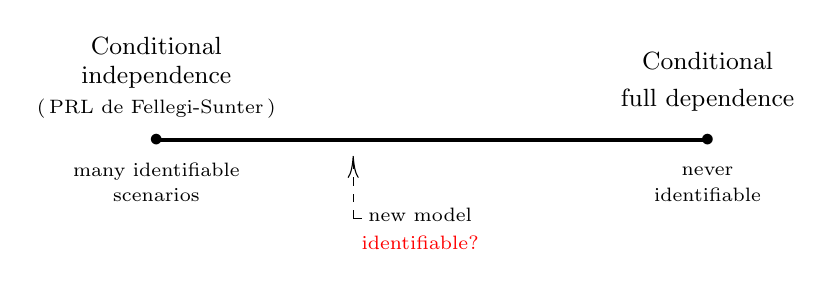
\begin{tikzpicture}
	%\draw[dashed,-{>[scale=2,length=4,width=2]}] (0,0) -- (0,2.85);
	%\draw[line width=0.05cm,{<[scale=2,length=4,width=4]}-{>[scale=2,length=4,width=4]}] (0,0) -- (9,0);
	\draw[line width=0.05cm] (0,0) -- (7,0);
	%%%%% ~~~~~ %%%%%
	\node at (0,0) {$\bullet$};
	\node at (0,1.2) {\small Conditional};
	\node at (0,0.8) {\small independence};
	\node at (0,0.4) {\scriptsize (\,PRL de Fellegi-Sunter\,)};
	\node at (0,-0.4) {\scriptsize many identifiable};
	\node at (0,-0.7) {\scriptsize scenarios};
	%%%%% ~~~~~ %%%%%
	\node at (7,0) {$\bullet$};
	\node at (7,1.0) {\small Conditional};
	\node at (7,0.5) {\small full dependence};
	\node at (7,-0.4) {\scriptsize never};
	\node at (7,-0.7) {\scriptsize identifiable};
	%%%%% ~~~~~ %%%%%
	\pause
	\draw[dashed,-{>[scale=2,length=4,width=2]}] (2.5,-1.0) -- (2.5,-0.2);
	\draw[dashed] (2.5,-1.0) -- (2.7,-1.0);
	\node at (3.35,-0.95) {\scriptsize new model};
	\pause
	\node at (3.35,-1.3) {\color{red}\scriptsize identifiable?};
\end{tikzpicture}
\end{center}


\vskip -0.5cm

\onslide<6->{
\footnotesize\begin{equation*}
\begin{array}{cccccl}
	\Psi \, : &
	{\color{red}\xcancel{\color{black}
		\left(\Delta_{d_{1}} \times \cdots \times \Delta_{d_{p}}\right)
		\times
		\left(\Delta_{d_{1}} \times \cdots \times \Delta_{d_{p}}\right)
		\times
		\Delta_{1}
	}}
	&\longrightarrow&
	{\color{red}\xcancel{\color{black}\underset{{\color{white}.}}{\overset{{\color{white}.}}{\mathcal{S}^{2}}}\!\left(\,\Sigma\,\right)}}
	&\subset&
	\Delta_{N}
\end{array}
\end{equation*}
}
\scriptsize
\begin{itemize}
\item
	\onslide<7->{No conditional independence,}
	\onslide<8->{no Segre varieties, nor their secant varieties.}
	%\onslide<7->{Sans ind\'ependance conditionelle,}
	%\onslide<8->{pas de vari\'et\'es de Segre non plus, ni ses vari\'et\'es de s\'ecantes non plus.}
\item
	\onslide<9->{Results of Catalisano \textit{et al.} and Allman \textit{et al.} no longer apply.}
	%\onslide<9->{Les r\'esultats de Catalisano \textit{et al.} et Allman \textit{et al.} ne sont plus applicables.}
\item
	\onslide<10->{Resulting parametrization maps may have never been studied in algebraic geometry.}
	%\onslide<10->{Les applications de param\'etrisation r\'esultantes n'ont peut-\^etre jamais \'et\'e \'etudi\'ees
	%en g\'eom\'etrie alg\'ebrique.}
\end{itemize}

\end{frame}
\normalsize

%%%%%%%%%%%%%%%%%%%%%%%%%%%%%%%%%%%%%%%%%%%%%%%%%%

%
\newcommand{\poz}{{\color{red}p^{(1)}_{0}}}
\newcommand{\poo}{{\color{red}p^{(1)}_{1}}}
\newcommand{\pot}{{\color{red}p^{(1)}_{2}}}

\newcommand{\ptz}{{\color{blue}p^{(2)}_{0}}}
\newcommand{\pto}{{\color{blue}p^{(2)}_{1}}}

\newcommand{\phz}{{\color{green}p^{(3)}_{0}}}
\newcommand{\pho}{{\color{green}p^{(3)}_{1}}}

\newcommand{\pozz}{{\color{red}p^{(1)}_{0|0}}}
\newcommand{\pooz}{{\color{red}p^{(1)}_{1|0}}}

\newcommand{\ptzz}{{\color{blue}p^{(2)}_{0|0}}}
\newcommand{\ptoz}{{\color{blue}p^{(2)}_{1|0}}}

\newcommand{\phzz}{{\color{green}p^{(3)}_{0|0}}}
\newcommand{\phoz}{{\color{green}p^{(3)}_{1|0}}}

\newcommand{\pozo}{{\color{pink}p^{(1)}_{0|1}}}
\newcommand{\pooo}{{\color{pink}p^{(1)}_{1|1}}}

\newcommand{\ptzo}{{\color{cyan}p^{(2)}_{0|1}}}
\newcommand{\ptoo}{{\color{cyan}p^{(2)}_{1|1}}}

\newcommand{\phzo}{{\color{lime}p^{(3)}_{0|1}}}
\newcommand{\phoo}{{\color{lime}p^{(3)}_{1|1}}}

%%%%%%%%%%%%%%%%%%%%%%%%%%%%%%%%%%%%%%%%%%%%%%%%%%
\begin{frame}{\Large Parameter space of categorical distributions = Probability simplex}

\begin{multicols}{2}

\begin{minipage}{5cm}
\vskip 1.5cm
\begin{equation*}
\begin{array}{c}
P(X=x_{1}) \;=\; \theta_{1} \\
P(X=x_{2}) \;=\; \theta_{2}
\end{array}
\end{equation*}
\end{minipage}

\newpage

\begin{minipage}{3cm}
\begin{flushright}
\input{z-one-simplex.tex}
\end{flushright}
\end{minipage}

\end{multicols}

\vskip -0.2cm
\begin{equation*}
\Delta_{\color{red}1}
\; := \;
\left\{\;
(\theta_{1},\theta_{2}) \in \Re^{2}
\;\;\left\vert\;
\begin{array}{c}
	0 \;\leq\; \theta_{1}, \theta_{2} \;\leq\; 1 \\
	\theta_{1} + \theta_{2} \;=\; 1
\end{array}
\right.
\right\}
\end{equation*}

\end{frame}
\normalsize

%%%%%%%%%%%%%%%%%%%%%%%%%%%%%%%%%%%%%%%%%%%%%%%%%%
\begin{frame}{\Large Parameter space of categorical distributions = Probability simplex (cont'd)}

\begin{multicols}{2}

\begin{minipage}{5cm}
\vskip 1.5cm
\begin{equation*}
\begin{array}{c}
P(X=x_{1}) \;=\; \theta_{1} \\
P(X=x_{2}) \;=\; \theta_{2} \\
P(X=x_{3}) \;=\; \theta_{3}
\end{array}
\end{equation*}
\end{minipage}

\newpage

\begin{minipage}{5cm}
\begin{center}
\includegraphics[width=4.5cm]{z-two-simplex.png}
\end{center}
\end{minipage}

\end{multicols}

\vskip -0.2cm
\begin{equation*}
\Delta_{\color{red}2}
\; := \;
\left\{\;
(\theta_{1},\theta_{2},\theta_{3}) \in \Re^{3}
\;\;\left\vert\;
\begin{array}{c}
	0 \;\leq\; \theta_{1}, \theta_{2}, \theta_{3} \;\leq\; 1 \\
	\theta_{1} + \theta_{2} + \theta_{3} \;=\; 1
\end{array}
\right.
\right\}
\end{equation*}

\end{frame}
\normalsize

%%%%%%%%%%%%%%%%%%%%%%%%%%%%%%%%%%%%%%%%%%%%%%%%%%
\begin{frame}{\Large Parameter space of categorical distributions = Probability simplex (cont'd)}

\begin{multicols}{2}

\begin{minipage}{5cm}
\vskip 1.0cm
\begin{equation*}
\begin{array}{c}
P(X=x_{1}) \;=\; \theta_{1} \\
P(X=x_{2}) \;=\; \theta_{2} \\
P(X=x_{3}) \;=\; \theta_{3} \\
P(X=x_{4}) \;=\; \theta_{4}
\end{array}
\end{equation*}
\end{minipage}

\newpage

\begin{minipage}{5cm}
\begin{center}
\includegraphics[width=3.5cm]{z-three-simplex.png}
\end{center}
\end{minipage}

\end{multicols}

\vskip -0.4cm
\begin{equation*}
\Delta_{\color{red}3}
\; := \;
\left\{\;
(\theta_{1},\theta_{2},\theta_{3},\theta_{4}) \in \Re^{4}
\;\;\left\vert\;
\begin{array}{c}
	0 \;\leq\; \theta_{1}, \theta_{2}, \theta_{3}, \theta_{4} \;\leq\; 1 \\
	\theta_{1} + \theta_{2} + \theta_{3} + \theta_{4} \;=\; 1
\end{array}
\right.
\right\}
\end{equation*}

\end{frame}
\normalsize

%%%%%%%%%%%%%%%%%%%%%%%%%%%%%%%%%%%%%%%%%%%%%%%%%%
\begin{frame}{\LARGE Contingency tables with independent factors \& Segre embeddings}

\begin{multicols}{2}

\scriptsize

\begin{minipage}{5cm}
\mbox{}
\begin{center}
\vskip 0.1cm
\begin{tabular}{|c||c|c||c|}
\hline
&&& \\
& $\textnormal{\tiny$X^{(2)} = 0$}$ & $\textnormal{\tiny$X^{(2)} = 1$}$ & \\
&&& \\
\hline\hline
&&& \\
$\textnormal{\tiny$X^{(1)} = 0$}$ & $\pi_{00}$ & $\pi_{01}$ & $\poz$ \\
&&& \\
\hline
&&& \\
$\textnormal{\tiny$X^{(1)} = 1$}$ & $\pi_{10}$ & $\pi_{11}$ & $\poo$ \\
&&& \\
\hline\hline
&&& \\
& $\ptz$ & $\pto$ & \\
&&& \\
\hline
\end{tabular}
\end{center}
\end{minipage}

\newpage

\pause

\begin{minipage}{5cm}

\begin{equation*}
f \; : \; {\color{red}\Delta_{1}} \times {\color{blue}\Delta_{1}} \;\longrightarrow\; \Sigma \, \subset \, \Delta_{3}
\end{equation*}

\tiny
\begin{eqnarray*}
	\overset{\Delta_{3}}{\overbrace{
	\left(\begin{array}{c}
	\overset{{\color{white}+}}{\pi}_{00} \\
	\overset{{\color{white}+}}{\pi}_{01} \\
	\overset{{\color{white}+}}{\pi}_{10} \\
	\overset{{\color{white}+}}{\pi}_{11}
	\end{array}\right)
	}}
& = &
	f\left(
		\left(\poz:\poo\right),
		\left(\ptz:\pto\right)
	\right)
\\
& = &
	\underset{\Sigma\,\subset\,\Delta_{3}}{\underbrace{
	\left(\begin{array}{c}
	\poz\,\ptz \\
	\poz\,\overset{{\color{white}.}}{\pto} \\
	\poo\,\overset{{\color{white}.}}{\ptz} \\
	\poo\,\overset{{\color{white}.}}{\pto}
	\end{array}\right)
	}}
\end{eqnarray*}
\end{minipage}

\end{multicols}

\end{frame}
\normalsize

%%%%%%%%%%%%%%%%%%%%%%%%%%%%%%%%%%%%%%%%%%%%%%%%%%
\begin{frame}{\LARGE Contingency tables with independent factors \& Segre embeddings (cont'd)}

\begin{equation*}
f \; : \; {\color{red}\Delta_{1}} \times {\color{blue}\Delta_{1}} \times {\color{green}\Delta_{1}} \;\longrightarrow\; \Sigma \, \subset \, \Delta_{7}
\end{equation*}

\vskip -0.3cm

\tiny
\begin{eqnarray*}
	\overset{\Delta_{7}}{\overbrace{
	\left(\begin{array}{c}
	\overset{{\color{white}+}}{\pi}_{000} \\
	\overset{{\color{white}+}}{\pi}_{001} \\
	\overset{{\color{white}+}}{\pi}_{010} \\
	\overset{{\color{white}+}}{\pi}_{011} \\
	\\
	\overset{{\color{white}+}}{\pi}_{100} \\
	\overset{{\color{white}+}}{\pi}_{101} \\
	\overset{{\color{white}+}}{\pi}_{110} \\
	\overset{{\color{white}+}}{\pi}_{111} \\
	\end{array}\right)
	}}
& = &
	f\left(
		\left(\poz:\poo\right),
		\left(\ptz:\pto\right),
		\left(\phz:\pho\right)
	\right)
\;\; = \;\;
	\overset{\Sigma\,\subset\,\Delta_{7}}{\overbrace{
	\left(\begin{array}{c}
	\poz\,\ptz\,\phz \\
	\poz\,\overset{{\color{white}.}}{\ptz}\,\pho \\
	\poz\,\overset{{\color{white}.}}{\pto}\,\phz \\
	\poz\,\overset{{\color{white}.}}{\pto}\,\pho \\
	\\
	\poo\,\overset{{\color{white}.}}{\ptz}\,\phz \\
	\poo\,\overset{{\color{white}.}}{\ptz}\,\pho \\
	\poo\,\overset{{\color{white}.}}{\pto}\,\phz \\
	\poo\,\overset{{\color{white}.}}{\pto}\,\pho
	\end{array}\right)
	}}
\end{eqnarray*}

\end{frame}
\normalsize

%%%%%%%%%%%%%%%%%%%%%%%%%%%%%%%%%%%%%%%%%%%%%%%%%%
\begin{frame}{\LARGE Contingency tables with independent factors \& Segre embeddings (cont'd)}

\vskip -0.1cm

\scriptsize
\begin{equation*}
	f
	\; : \;
	{\color{red}\Delta_{2}} \times {\color{blue}\Delta_{1}} \times {\color{green}\Delta_{1}}
	\;\longrightarrow\;
	\Sigma \, \subset \, \Delta_{11} \,=\, \Delta_{3 \times 2 \times 2 - 1}
\end{equation*}

\vskip -0.5cm

\tiny
\begin{eqnarray*}
	\overset{\Delta_{11}}{\overbrace{
	\left(\begin{array}{c}
	\overset{{\color{white}+}}{\pi}_{000} \\
	\overset{{\color{white}+}}{\pi}_{001} \\
	\overset{{\color{white}+}}{\pi}_{010} \\
	\overset{{\color{white}+}}{\pi}_{011} \\
	\\
	\overset{{\color{white}+}}{\pi}_{100} \\
	\overset{{\color{white}+}}{\pi}_{101} \\
	\overset{{\color{white}+}}{\pi}_{110} \\
	\overset{{\color{white}+}}{\pi}_{111} \\
	\\
	\overset{{\color{white}+}}{\pi}_{200} \\
	\overset{{\color{white}+}}{\pi}_{201} \\
	\overset{{\color{white}+}}{\pi}_{210} \\
	\overset{{\color{white}+}}{\pi}_{211} \\
	\end{array}\right)
	}}
& = &
	f\left(
		\left(\poz:\poo:\pot\right),
		\left(\ptz:\pto\right),
		\left(\phz:\pho\right)
	\right)
\;\; = \;\;
	\overset{\Sigma\,\subset\,\Delta_{11}}{\overbrace{
	\left(\begin{array}{c}
	\poz\,\ptz\,\phz \\
	\poz\,\overset{{\color{white}.}}{\ptz}\,\pho \\
	\poz\,\overset{{\color{white}.}}{\pto}\,\phz \\
	\poz\,\overset{{\color{white}.}}{\pto}\,\pho \\
	\\
	\poo\,\overset{{\color{white}.}}{\ptz}\,\phz \\
	\poo\,\overset{{\color{white}.}}{\ptz}\,\pho \\
	\poo\,\overset{{\color{white}.}}{\pto}\,\phz \\
	\poo\,\overset{{\color{white}.}}{\pto}\,\pho \\
	\\
	\pot\,\overset{{\color{white}.}}{\ptz}\,\phz \\
	\pot\,\overset{{\color{white}.}}{\ptz}\,\pho \\
	\pot\,\overset{{\color{white}.}}{\pto}\,\phz \\
	\pot\,\overset{{\color{white}.}}{\pto}\,\pho
	\end{array}\right)
	}}
\end{eqnarray*}

\end{frame}
\normalsize

%%%%%%%%%%%%%%%%%%%%%%%%%%%%%%%%%%%%%%%%%%%%%%%%%%
\begin{frame}{\Large \vskip -0.3cm Latent Class Models for Contingency Tables \&\vskip 0.1cm Fellegi-Sunter Probabilistic Record Linkage}

\tiny

\pause
\vskip -0.25cm
\begin{eqnarray*}
\pi_{\gamma}
& = & P\!\left(\,\Gamma = \gamma\,\right)
\;\; = \;\;
	P\!\left(\,\Gamma = \gamma\;\vert\;M=1\,\right)\cdot P\!\left(\,M=1\,\right)
	\; + \;
	P\!\left(\,\Gamma = \gamma\;\vert\;M=0\,\right)\cdot P\!\left(\,M=0\,\right)
\\
& = &
	\overset{1}{\underset{m=0}{\sum}}\;
	P\!\left(\,M=m\,\right) \cdot
	\overset{p}{\underset{i=1}{\prod}}\;P\!\left(\,\Gamma_{i} = \gamma_{i}\;\vert\,M=m\,\right)
\end{eqnarray*}

\pause
\scriptsize
\begin{eqnarray*}
\pi_{000} &=& \pozz\,\ptzz\,\phzz \cdot q_{0} \;+\; \pozo\,\ptzo\,\phzo \cdot q_{1} \\
\pi_{001} &=& \pozz\,\ptzz\,\phoz \cdot q_{0} \;+\; \pozo\,\ptzo\,\phoo \cdot q_{1} \\
\pi_{010} &=& \pozz\,\ptoz\,\phzz \cdot q_{0} \;+\; \pozo\,\ptoo\,\phzo \cdot q_{1} \\
\pi_{011} &=& \pozz\,\ptoz\,\phoz \cdot q_{0} \;+\; \pozo\,\ptoo\,\phoo \cdot q_{1} \\
\pi_{100} &=& \pooz\,\ptzz\,\phzz \cdot q_{0} \;+\; \pooo\,\ptzo\,\phzo \cdot q_{1} \\
\pi_{101} &=& \pooz\,\ptzz\,\phoz \cdot q_{0} \;+\; \pooo\,\ptzo\,\phoo \cdot q_{1} \\
\pi_{110} &=& \pooz\,\ptoz\,\phzz \cdot q_{0} \;+\; \pooo\,\ptoo\,\phzo \cdot q_{1} \\
\pi_{111} &=& \pooz\,\ptoz\,\phoz \cdot q_{0} \;+\; \pooo\,\ptoo\,\phoo \cdot q_{1} \\
\end{eqnarray*}

%\begin{equation*}
%\log P\!\left(\,Y = y\,\right)
%\;\; = \;\;
%\underset{\gamma\,\in\,\mathcal{G}}{\textnormal{\large$\sum$}}\;\, y_{\gamma}\cdot
%	\log\!\left[\;
%		\overset{1}{\underset{m=0}{\sum}}\;
%		{\color{red}P\!\left(\,M=m\,\right)} \cdot
%		\overset{p}{\underset{i=1}{\prod}}\,{\color{red}P\!\left(\,\Gamma_{i} = \gamma_{i}\;\vert\,M=m\,\right)}
%	\;\right]
%\; + \;
%\log\!\left(n!\left/\overset{{\color{white}.}}{\underset{\gamma\,\in\,\mathcal{G}}{\prod}}\,y_{\gamma}!\right.\right),
%\end{equation*}

\end{frame}
\normalsize

%%%%%%%%%%%%%%%%%%%%%%%%%%%%%%%%%%%%%%%%%%%%%%%%%%
\begin{frame}{\Large \vskip -0.3cm Latent Class Models for Contingency Tables \&\vskip 0.1cm Fellegi-Sunter Probabilistic Record Linkage}

\vskip -0.3cm

\tiny
%\begin{eqnarray*}
%\pi_{000} &=& \pozz\,\ptzz\,\phzz \cdot q_{0} \;+\; \pozo\,\ptzo\,\phzo \cdot q_{1} \\
%\pi_{001} &=& \pozz\,\ptzz\,\phoz \cdot q_{0} \;+\; \pozo\,\ptzo\,\phoo \cdot q_{1} \\
%\pi_{010} &=& \pozz\,\ptoz\,\phzz \cdot q_{0} \;+\; \pozo\,\ptoo\,\phzo \cdot q_{1} \\
%\pi_{011} &=& \pozz\,\ptoz\,\phoz \cdot q_{0} \;+\; \pozo\,\ptoo\,\phoo \cdot q_{1} \\
%\pi_{100} &=& \pooz\,\ptzz\,\phzz \cdot q_{0} \;+\; \pooo\,\ptzo\,\phzo \cdot q_{1} \\
%\pi_{101} &=& \pooz\,\ptzz\,\phoz \cdot q_{0} \;+\; \pooo\,\ptzo\,\phoo \cdot q_{1} \\
%\pi_{110} &=& \pooz\,\ptoz\,\phzz \cdot q_{0} \;+\; \pooo\,\ptoo\,\phzo \cdot q_{1} \\
%\pi_{111} &=& \pooz\,\ptoz\,\phoz \cdot q_{0} \;+\; \pooo\,\ptoo\,\phoo \cdot q_{1} \\
%\end{eqnarray*}

\begin{eqnarray*}
\left(\begin{array}{c}
\overset{{\color{white}+}}{\pi}_{000} \\
\overset{{\color{white}+}}{\pi}_{001} \\
\overset{{\color{white}+}}{\pi}_{010} \\
\overset{{\color{white}+}}{\pi}_{011} \\
\overset{{\color{white}+}}{\pi}_{100} \\
\overset{{\color{white}+}}{\pi}_{101} \\
\overset{{\color{white}+}}{\pi}_{110} \\
\overset{{\color{white}+}}{\pi}_{111} \\
\end{array}\right)
& = &
\left(\begin{array}{c}
\pozz\,\ptzz\,\phzz \cdot q_{0} \;+\; \pozo\,\ptzo\,\phzo \cdot q_{1} \\
\pozz\,\ptzz\,\phoz \cdot q_{0} \;+\; \pozo\,\ptzo\,\phoo \cdot q_{1} \\
\pozz\,\ptoz\,\phzz \cdot q_{0} \;+\; \pozo\,\ptoo\,\phzo \cdot q_{1} \\
\pozz\,\ptoz\,\phoz \cdot q_{0} \;+\; \pozo\,\ptoo\,\phoo \cdot q_{1} \\
\pooz\,\ptzz\,\phzz \cdot q_{0} \;+\; \pooo\,\ptzo\,\phzo \cdot q_{1} \\
\pooz\,\ptzz\,\phoz \cdot q_{0} \;+\; \pooo\,\ptzo\,\phoo \cdot q_{1} \\
\pooz\,\ptoz\,\phzz \cdot q_{0} \;+\; \pooo\,\ptoo\,\phzo \cdot q_{1} \\
\pooz\,\ptoz\,\phoz \cdot q_{0} \;+\; \pooo\,\ptoo\,\phoo \cdot q_{1} \\
\end{array}\right)
\\
\pause
& = &
q_{0} \cdot
\left(\begin{array}{c}
\pozz\,\ptzz\,\phzz \\
\pozz\,\ptzz\,\phoz \\
\pozz\,\ptoz\,\phzz \\ 
\pozz\,\ptoz\,\phoz \\
\pooz\,\ptzz\,\phzz \\
\pooz\,\ptzz\,\phoz \\
\pooz\,\ptoz\,\phzz \\
\pooz\,\ptoz\,\phoz
\end{array}\right)
\;\; + \;\;
q_{1} \cdot
\left(\begin{array}{c}
\pozo\,\ptzo\,\phzo \\
\pozo\,\ptzo\,\phoo \\
\pozo\,\ptoo\,\phzo \\
\pozo\,\ptoo\,\phoo \\
\pooo\,\ptzo\,\phzo \\
\pooo\,\ptzo\,\phoo \\
\pooo\,\ptoo\,\phzo \\
\pooo\,\ptoo\,\phoo
\end{array}\right)
\end{eqnarray*}

\end{frame}
\normalsize

%%%%%%%%%%%%%%%%%%%%%%%%%%%%%%%%%%%%%%%%%%%%%%%%%%
\begin{frame}{\vskip -0.35cm \Large Model parametrization map of\\ Fellegi-Sunter Probabilistic Record Linkage}

\vskip -0.35cm

\tiny

\begin{eqnarray*}
	\overset{\Delta_{7}}{\overbrace{
	\left(\begin{array}{c}
	\overset{{\color{white}+}}{\pi}_{000} \\
	\overset{{\color{white}+}}{\pi}_{001} \\
	\overset{{\color{white}+}}{\pi}_{010} \\
	\overset{{\color{white}+}}{\pi}_{011} \\
	\overset{{\color{white}+}}{\pi}_{100} \\
	\overset{{\color{white}+}}{\pi}_{101} \\
	\overset{{\color{white}+}}{\pi}_{110} \\
	\overset{{\color{white}+}}{\pi}_{111} \\
	\end{array}\right)
	}}
& = &
q_{0} \cdot
	\overset{\Sigma\,\subset\,\Delta_{7}}{\overbrace{
	\left(\begin{array}{c}
	\pozz\,\ptzz\,\phzz \\
	\pozz\,\ptzz\,\phoz \\
	\pozz\,\ptoz\,\phzz \\ 
	\pozz\,\ptoz\,\phoz \\
	\pooz\,\ptzz\,\phzz \\
	\pooz\,\ptzz\,\phoz \\
	\pooz\,\ptoz\,\phzz \\
	\pooz\,\ptoz\,\phoz
	\end{array}\right)
	}}
\;\; + \;\;
q_{1} \cdot
	\overset{\Sigma\,\subset\,\Delta_{7}}{\overbrace{
	\left(\begin{array}{c}
	\pozo\,\ptzo\,\phzo \\
	\pozo\,\ptzo\,\phoo \\
	\pozo\,\ptoo\,\phzo \\
	\pozo\,\ptoo\,\phoo \\
	\pooo\,\ptzo\,\phzo \\
	\pooo\,\ptzo\,\phoo \\
	\pooo\,\ptoo\,\phzo \\
	\pooo\,\ptoo\,\phoo
	\end{array}\right)
	}}
\end{eqnarray*}

\pause
\vskip -0.5cm
\tiny
\begin{eqnarray*}
&&
	\left(\,\pi_{000}\,:\,\overset{{\color{white}|}}{\ldots}\,:\,\pi_{111}\,\right)
\\
&=&
	\Psi\left(\,
		\left(\pozz:\pooz\right),
		\left(\ptzz:\ptoz\right),
		\left(\phzz:\phoz\right),
		\left(\pozo:\pooo\right),
		\left(\ptzo:\ptoo\right),
		\left(\phzo:\phoo\right),
		\left(q_{0}:q_{1}\right)
	\,\right)
\end{eqnarray*}

\tiny
\begin{equation*}
\Psi \, :
\left({\color{red}\Delta_{1}} \overset{{\color{white}.}}{\times} {\color{blue}\Delta_{1}} \times {\color{green}\Delta_{1}}\right)
\times
\left({\color{pink}\Delta_{1}} \overset{{\color{white}.}}{\times} {\color{cyan}\Delta_{1}} \times {\color{lime}\Delta_{1}}\right)
\times
\Delta_{1}
\;\;\longrightarrow\;\;
\mathcal{S}^{2}\!\left(\,\Sigma\,\right) \,\subset\, \Delta_{7}
\end{equation*}

\pause

\scriptsize
\begin{equation*}
\Psi \, :
\left(\Delta_{d_{1}} \times \cdots \times \Delta_{d_{p}}\right)
\times \cdots \times
\left(\Delta_{d_{1}} \times \cdots \times \Delta_{d_{p}}\right)
\times
\Delta_{r-1}
\;\;\longrightarrow\;\;
\mathcal{S}^{r}\!\left(\,\Sigma\,\right) \,\subset\, \Delta_{d_{1}\cdots d_{p} - 1}
\end{equation*}

%\large
%\begin{center}
%\textbf{
%Identifiability
%\;$:=$\;
%generic injectivity of $\Psi$
%}
%\end{center}

\end{frame}
\normalsize

%%%%%%%%%%%%%%%%%%%%%%%%%%%%%%%%%%%%%%%%%%%%%%%%%%
\begin{frame}{\Large What is ``identifiability'' here, at least intuitively?}

\vskip -0.35cm

\scriptsize
\begin{equation*}
\Psi \, :
\left({\color{red}\Delta_{1}} \overset{{\color{white}.}}{\times} {\color{blue}\Delta_{1}} \times {\color{green}\Delta_{1}}\right)
\times
\left({\color{pink}\Delta_{1}} \overset{{\color{white}.}}{\times} {\color{cyan}\Delta_{1}} \times {\color{lime}\Delta_{1}}\right)
\times
\Delta_{1}
\;\;\longrightarrow\;\;
\mathcal{S}^{2}\!\left(\,\Sigma\,\right) \,\subset\, \Delta_{7}
\end{equation*}

\vskip -0.3cm

\tiny
\begin{eqnarray*}
&&
	\left(\,\pi_{000}\,:\,\overset{{\color{white}|}}{\ldots}\,:\,\pi_{111}\,\right)
\\
&=&
	\Psi\left(\,
		\left(\pozz:\pooz\right),
		\left(\ptzz:\ptoz\right),
		\left(\phzz:\phoz\right),
		\left(\pozo:\pooo\right),
		\left(\ptzo:\ptoo\right),
		\left(\phzo:\phoo\right),
		\left(q_{0}:q_{1}\right)
	\,\right)
\end{eqnarray*}

\pause

\vskip 0.6cm
\small
\begin{center}
\textbf{\Large Is \,$\Psi$\, ``identifiable''\,?}
\end{center}
\pause
\vskip 0.2cm
Does \;$\left(\,\pi_{000}\,:\,\overset{{\color{white}|}}{\ldots}\,:\,\pi_{111}\,\right)$\;
``uniquely determine''
\tiny
\begin{equation*}
\left(\,
	\left(\pozz:\pooz\right),
	\left(\ptzz:\ptoz\right),
	\left(\phzz:\phoz\right),
	\left(\pozo:\pooo\right),
	\left(\ptzo:\ptoo\right),
	\left(\phzo:\phoo\right),
	\left(q_{0}:q_{1}\right)
\,\right)?
\end{equation*}

%\large
%\begin{center}
%\textbf{
%Identifiability
%\;$:=$\;
%generic injectivity of $\Psi$
%}
%\end{center}

\end{frame}
\normalsize

%%%%%%%%%%%%%%%%%%%%%%%%%%%%%%%%%%%%%%%%%%%%%%%%%%

%
%%%%%%%%%%%%%%%%%%%%%%%%%%%%%%%%%%%%%%%%%%%%%%%%%%
\begin{frame}{\LARGE Identifiability of linear models}

\vskip 0.3cm

\pause
Data:{\scriptsize
\begin{equation*}
\begin{array}{c||c|c|c||c|c|c}
i & 1 & 2 & 3 & 4 & 5 & 6 \\
\hline\hline
x & \textnormal{A} & \textnormal{A} & \textnormal{A} &
      \textnormal{B} & \textnormal{B} & \textnormal{B}
\\
\hline
y & ? & ? & ? & ? & ? & ?
\end{array}
\end{equation*}
}

\vskip -0.25cm
\pause
\begin{equation*}
\begin{array}{llcccclc}
\textnormal{Model \;I:} \quad\mbox{}&
	y_{i} &=& \mu + \tau_{x_{i}} &+& \varepsilon_{i}, &
	E\left[\,\varepsilon_{i}\,\right] = 0, &
	\varepsilon_{i} \;\;\textnormal{i.i.d.} \\
\textnormal{Model II:}  \quad\mbox{}&
	y_{i} &\overset{{\color{white}\vert}}{=}& \alpha_{x_{i}} &+& \varepsilon_{i}, &
	E\left[\,\varepsilon_{i}\,\right] = 0, &
	\varepsilon_{i} \;\;\textnormal{i.i.d.}
\end{array}
\end{equation*}
where $\mu$, $\tau_{\textnormal{A}}$, $\tau_{\textnormal{B}}$,
are unknown \textbf{model parameters} of Model I (to be estimated based on data),
while $\alpha_{\textnormal{A}}$, $\alpha_{\textnormal{B}}$ those of Model II.

%\vskip 0.5cm
%\pause
%Assumption:\quad
%$E\!\left[\,y_{i}\,\right]$ fully determines probability distribution of $y_{i}$.

\vskip 0.8cm
\pause
{\Large\color{customRed}Fact:\quad Model I \;is NOT identifiable; \; Model II \;is.}

\end{frame}
\normalsize

%%%%%%%%%%%%%%%%%%%%%%%%%%%%%%%%%%%%%%%%%%%%%%%%%%

\begin{frame}{\LARGE Identifiability of linear models (cont'd)}

\pause
{\tiny
\begin{equation*}
\begin{array}{c||c|c|c||c|c|c}
i & 1 & 2 & 3 & 4 & 5 & 6 \\
\hline\hline
x & \textnormal{A} & \textnormal{A} & \textnormal{A} &
      \textnormal{B} & \textnormal{B} & \textnormal{B}
\\
\hline
y & ? & ? & ? & ? & ? & ?
\end{array}
\quad
\quad
\quad
\begin{array}{lccl}
	M_{\textnormal{I}}: & y_{i} &=& \mu + \tau_{x_{i}} + \varepsilon_{i}
	\\ \\
	M_{\textnormal{II}}: & y_{i} &=& \mbox{}\quad{\color{customRed}\alpha_{x_{i}}}\quad\mbox{} + \varepsilon_{i}
\end{array}\,,
\quad
\quad
\quad
\begin{array}{c}
	\varepsilon_{i} \;\; \textnormal{i.i.d.}
	\\
	\overset{{\color{white}-}}{E}\!\left[\,\varepsilon_{i}\,\right] = 0
\end{array}
\end{equation*}
}

\vskip -0.5cm

\pause
{\tiny
\begin{eqnarray*}
\left(\begin{array}{c}
	E\!\left[\,y_{1}\,\right] \\ E\!\left[\,y_{2}\,\right] \\ E\!\left[\,y_{3}\,\right] \\
	E\!\left[\,{\color{customRed}y_{4}}\,\right] \\ E\!\left[\,{\color{customRed}y_{5}}\,\right] \\ E\!\left[\,{\color{customRed}y_{6}}\,\right]
	\end{array}\right)
&=&
\left(\begin{array}{c}
	\mu + \tau_{\textnormal{A}} \\	\mu + \tau_{\textnormal{A}} \\ 	\mu + \tau_{\textnormal{A}} \\
	\mu + \tau_{\color{customRed}\textnormal{B}} \\
	\mu + \tau_{\color{customRed}\textnormal{B}} \\ 
	\mu + \tau_{\color{customRed}\textnormal{B}}
	\end{array}\right)
\\
\pause
&=&
\mu\left(\begin{array}{c} 1\\1\\1\\1\\1\\1 \end{array}\right)
\;+\;\tau_{\textnormal{A}}\left(\begin{array}{c} 1\\1\\1\\0\\0\\0 \end{array}\right)
\;+\;\tau_{\textnormal{B}}\left(\begin{array}{c} 0\\0\\0\\1\\1\\1 \end{array}\right)
\pause
\;=\;
\left[\begin{array}{cccc}
	1&1&0\\
	1&1&0\\
	1&1&0\\
	1&0&1\\
	1&0&1\\
	1&0&1
\end{array}\right]
\left(\!\begin{array}{l} \mu \\ \tau_{\textnormal{A}} \\ \tau_{\textnormal{B}} \end{array}\!\!\right)
%\;=\;
%X\cdot\!
%\left(\!\begin{array}{l} \mu \\ \tau_{\textnormal{A}} \\ \tau_{\textnormal{B}} \end{array}\!\!\right)
\\
\pause
&=&
      (\mu+\tau_{\textnormal{A}})\left(\begin{array}{c} 1\\1\\1\\0\\0\\0 \end{array}\right)
\;+\;(\mu+\tau_{\textnormal{B}})\left(\begin{array}{c} 0\\0\\0\\1\\1\\1 \end{array}\right)
\pause
\;=\;
\left[\begin{array}{cccc}
	1&0\\
	1&0\\
	1&0\\
	0&1\\
	0&1\\
	0&1
\end{array}\right]
\left(\!\begin{array}{l} \mu + \tau_{\textnormal{A}} \\ \mu + \tau_{\textnormal{B}} \end{array}\!\!\right)
%\;=\;
%X\cdot\!
%\left(\!\begin{array}{l} \mu + \tau_{\textnormal{A}} \\ \mu + \tau_{\textnormal{B}} \end{array}\!\!\right)
\end{eqnarray*}
}

\end{frame}
\normalsize

%%%%%%%%%%%%%%%%%%%%%%%%%%%%%%%%%%%%%%%%%%%%%%%%%%

\begin{frame}{\LARGE Identifiability of linear models (cont'd)}

\vskip -0.2cm


\begin{minipage}{4in}
{\tiny
\begin{equation*}
\begin{array}{c||c|c|c||c|c|c}
i & 1 & 2 & 3 & 4 & 5 & 6 \\
\hline\hline
x & \textnormal{A} & \textnormal{A} & \textnormal{A} &
      \textnormal{B} & \textnormal{B} & \textnormal{B}
\\
\hline
y & ? & ? & ? & ? & ? & ?
\end{array}
\quad
\quad
\quad
\begin{array}{lccl}
	M_{\textnormal{I}}: & y_{i} &=& \mu + \tau_{x_{i}} + \varepsilon_{i}
	\\
	\overset{{\color{white}-}}{M}_{\textnormal{II}}: & y_{i} &=& \mbox{}\quad{\color{customRed}\alpha_{x_{i}}}\quad\mbox{} + \varepsilon_{i}
\end{array}\,,
\quad
\quad
\quad
\begin{array}{c}
	\varepsilon_{i} \;\; \textnormal{i.i.d.}
	\\
	\overset{{\color{white}-}}{E}\!\left[\,\varepsilon_{i}\,\right] = 0
\end{array}
\end{equation*}
}

\vskip -0.7cm

{\tiny
\begin{eqnarray*}
\left(\begin{array}{c}
	E\!\left[\,y_{1}\,\right] \\ E\!\left[\,y_{2}\,\right] \\ E\!\left[\,y_{3}\,\right] \\
	E\!\left[\,{\color{customRed}y_{4}}\,\right] \\ E\!\left[\,{\color{customRed}y_{5}}\,\right] \\ E\!\left[\,{\color{customRed}y_{6}}\,\right]
	\end{array}\right)
&=&
\underset{X_{\textnormal{I}}}{\underbrace{\left[\begin{array}{cccc}
	1&1&0\\
	1&1&0\\
	1&1&0\\
	1&0&1\\
	1&0&1\\
	1&0&1
\end{array}\right]}}
\left(\!\begin{array}{l} \mu \\ \tau_{\textnormal{A}} \\ \tau_{\textnormal{B}} \end{array}\!\!\right)
%\;=\;
%X\cdot\!
%\left(\!\begin{array}{l} \mu \\ \tau_{\textnormal{A}} \\ \tau_{\textnormal{B}} \end{array}\!\!\right)
\;\;=\;\;
\left[\begin{array}{cccc}
	1&0\\
	1&0\\
	1&0\\
	0&1\\
	0&1\\
	0&1
\end{array}\right]
\left(\!\begin{array}{l} \mu + \tau_{\textnormal{A}} \\ \mu + \tau_{\textnormal{B}} \end{array}\!\!\right)
%\;=\;
%X\cdot\!
%\left(\!\begin{array}{l} \mu + \tau_{\textnormal{A}} \\ \mu + \tau_{\textnormal{B}} \end{array}\!\!\right)
\;\;=\;\;
\underset{X_{\textnormal{II}}}{\underbrace{\left[\begin{array}{cccc}
	1&0\\
	1&0\\
	1&0\\
	0&1\\
	0&1\\
	0&1
\end{array}\right]}}
\left(\!\begin{array}{l} \alpha_{\textnormal{A}} \\ \alpha_{\textnormal{B}} \end{array}\!\!\right)
\end{eqnarray*}
}
\end{minipage}


\vskip -0.3cm

Recall (least-squares estimators):\pause
{\scriptsize
\begin{equation*}
\left(\!\begin{array}{l}
	\widehat{\mu} \\
	\overset{{\color{white}.}}{\widehat{\tau}_{\textnormal{A}}} \\
	\overset{{\color{white}.}}{\widehat{\tau}_{\textnormal{B}}}
\end{array}\!\!\right)
\;\;=\;\;
\left(X_{\textnormal{I}}^{T}X_{\textnormal{I}}\right)^{-1}X_{\textnormal{I}}^{T}\cdot\mathbf{y}\,,
\quad\quad
\textnormal{and}
\quad\quad
\left(\!\begin{array}{l}
	\overset{{\color{white}.}}{\widehat{\alpha}_{\textnormal{A}}} \\
	\overset{{\color{white}.}}{\widehat{\alpha}_{\textnormal{B}}}
\end{array}\!\!\right)
\;\;=\;\;
\left(X_{\textnormal{II}}^{T}X_{\textnormal{II}}\right)^{-1}X_{\textnormal{II}}^{T}\cdot\mathbf{y}\,,
\end{equation*}
}\pause
except that \pause\,$X_{\textnormal{I}}^{T}X_{\textnormal{I}}$\, is NOT invertible
\pause(cannot solve for\, $\widehat{\mu}$,\, $\widehat{\tau}_{\textnormal{A}}$,\, $\widehat{\tau}_{\textnormal{B}}$\,;
\pause \textbf{Model I is not identifiable}),
\pause
since the design matrix \,$X_{\textnormal{I}}$\, does not have full rank.

\end{frame}
\normalsize

%%%%%%%%%%%%%%%%%%%%%%%%%%%%%%%%%%%%%%%%%%%%%%%%%%

\begin{frame}{\LARGE Identifiability of linear models (cont'd)}

\vskip -0.35cm


\begin{minipage}{4in}
{\tiny
\begin{equation*}
\begin{array}{c||c|c|c||c|c|c}
i & 1 & 2 & 3 & 4 & 5 & 6 \\
\hline\hline
x & \textnormal{A} & \textnormal{A} & \textnormal{A} &
      \textnormal{B} & \textnormal{B} & \textnormal{B}
\\
\hline
y & ? & ? & ? & ? & ? & ?
\end{array}
\quad
\quad
\quad
\begin{array}{lccl}
	M_{\textnormal{I}}: & y_{i} &=& \mu + \tau_{x_{i}} + \varepsilon_{i}
	\\
	\overset{{\color{white}-}}{M}_{\textnormal{II}}: & y_{i} &=& \mbox{}\quad{\color{customRed}\alpha_{x_{i}}}\quad\mbox{} + \varepsilon_{i}
\end{array}\,,
\quad
\quad
\quad
\begin{array}{c}
	\varepsilon_{i} \;\; \textnormal{i.i.d.}
	\\
	\overset{{\color{white}-}}{E}\!\left[\,\varepsilon_{i}\,\right] = 0
\end{array}
\end{equation*}
}

\vskip -0.7cm

{\tiny
\begin{eqnarray*}
\left(\begin{array}{c}
	E\!\left[\,y_{1}\,\right] \\ E\!\left[\,y_{2}\,\right] \\ E\!\left[\,y_{3}\,\right] \\
	E\!\left[\,{\color{customRed}y_{4}}\,\right] \\ E\!\left[\,{\color{customRed}y_{5}}\,\right] \\ E\!\left[\,{\color{customRed}y_{6}}\,\right]
	\end{array}\right)
&=&
\underset{X_{\textnormal{I}}}{\underbrace{\left[\begin{array}{cccc}
	1&1&0\\
	1&1&0\\
	1&1&0\\
	1&0&1\\
	1&0&1\\
	1&0&1
\end{array}\right]}}
\left(\!\begin{array}{l} \mu \\ \tau_{\textnormal{A}} \\ \tau_{\textnormal{B}} \end{array}\!\!\right)
%\;=\;
%X\cdot\!
%\left(\!\begin{array}{l} \mu \\ \tau_{\textnormal{A}} \\ \tau_{\textnormal{B}} \end{array}\!\!\right)
\;\;=\;\;
\left[\begin{array}{cccc}
	1&0\\
	1&0\\
	1&0\\
	0&1\\
	0&1\\
	0&1
\end{array}\right]
\left(\!\begin{array}{l} \mu + \tau_{\textnormal{A}} \\ \mu + \tau_{\textnormal{B}} \end{array}\!\!\right)
%\;=\;
%X\cdot\!
%\left(\!\begin{array}{l} \mu + \tau_{\textnormal{A}} \\ \mu + \tau_{\textnormal{B}} \end{array}\!\!\right)
\;\;=\;\;
\underset{X_{\textnormal{II}}}{\underbrace{\left[\begin{array}{cccc}
	1&0\\
	1&0\\
	1&0\\
	0&1\\
	0&1\\
	0&1
\end{array}\right]}}
\left(\!\begin{array}{l} \alpha_{\textnormal{A}} \\ \alpha_{\textnormal{B}} \end{array}\!\!\right)
\end{eqnarray*}
}
\end{minipage}


\vskip -0.3cm

\newcommand{\colSpace}{\textnormal{colSpace}}

In terms of \textbf{model parametrization maps}:\pause
{\scriptsize
\vskip -0.6cm
\begin{equation*}
\begin{array}{lclclcccc}
\varphi_{\textnormal{I}} &: &\Re^{3} &\longrightarrow& M \,=\, \colSpace\!\left(X_{\textnormal{I}}\right) \,\subset\, \Re^{6}
&:&
\textnormal{\tiny$\left(\!\begin{array}{l} \mu \\ \tau_{\textnormal{A}} \\ \tau_{\textnormal{B}} \end{array}\!\!\right)$}
&\longmapsto&
X_{\textnormal{I}}
\textnormal{\tiny$\left(\!\begin{array}{l} \mu \\ \tau_{\textnormal{A}} \\ \tau_{\textnormal{B}} \end{array}\!\!\right)$}
\\
\pause
\varphi_{\textnormal{II}} &: & \Re^{2} &\longrightarrow& M \,=\, \colSpace\!\left(X_{\textnormal{II}}\right) \subset\, \Re^{6}
&\overset{{\color{white}\vert}}{:}&
\textnormal{\tiny$\left(\!\begin{array}{l} \alpha_{\textnormal{A}} \\ \alpha_{\textnormal{B}} \end{array}\!\!\right)$}
&\longmapsto&
X_{\textnormal{II}}
\textnormal{\tiny$\left(\!\begin{array}{l} \alpha_{\textnormal{A}} \\ \alpha_{\textnormal{B}} \end{array}\!\!\right)$}
\end{array}
\end{equation*}
}\pause
Note:\quad
\textbf{$\varphi_{\textnormal{I}}$\; is not injective (one-to-one), \quad\; \pause while \;$\varphi_{\textnormal{II}}$\; is.}
\vskip 0.1cm
\pause
{\color{white}Note:}\quad\quad\textbf{Model I\; is not identifiable, \;\; while \;Model II\; is.}

\end{frame}
\normalsize

%%%%%%%%%%%%%%%%%%%%%%%%%%%%%%%%%%%%%%%%%%%%%%%%%%

\begin{frame}{\LARGE Identifiability of linear models (cont'd)}

\large
Linear \textbf{models} can be regarded as linear \textbf{maps}
\pause
{\LARGE
\begin{equation*}
\begin{array}{clcll}
{\color{customRed}\varphi} : & {\color{customRed}\Theta} = \Re^{p} & \longrightarrow & M & \subset {\color{customRed}\Psi} = \Re^{n} \\
& \beta & \longmapsto & X\cdot\beta & (X \in \Re^{n\times p})
\end{array}
\end{equation*}
}
between
\pause
\begin{center}\vskip 0.2cm{\LARGE finite-dimensional vector spaces.}\end{center}

\pause
\vskip 0.5cm
\textbf{Identifiability} of linear models is simply:
\pause
\begin{center}{\LARGE\textbf{injectivity} of these linear maps.}\end{center}

\end{frame}
\normalsize

%%%%%%%%%%%%%%%%%%%%%%%%%%%%%%%%%%%%%%%%%%%%%%%%%%

%
%%%%%%%%%%%%%%%%%%%%%%%%%%%%%%%%%%%%%%%%%%%%%%%%%%
\begin{frame}{\Large Sufficient conditions for generic identifiability}

\scriptsize
\begin{equation*}
\Psi \, :
\left(\Delta_{d_{1}} \times \cdots \times \Delta_{d_{p}}\right)
\times \cdots \times
\left(\Delta_{d_{1}} \times \cdots \times \Delta_{d_{p}}\right)
\times
\Delta_{r-1}
\;\;\longrightarrow\;\;
\mathcal{S}^{r}\!\left(\,\Sigma\,\right) \,\subset\, \Delta_{d_{1}\cdots d_{p} - 1}
\end{equation*}

\pause
\scriptsize
\vskip 0.5cm
Allman-Matias-Rhodes (2009) introduced the notion of \textbf{\color{red}generic identifiability} and
gave sufficient conditions on $r, d_{1}, d_{2}, \cdots, d_{p}$ for $\Psi$ to be generically identifiable.

\pause
\vskip 0.5cm
\scriptsize
\textbf{Corollary 3, Allman \textit{et al.} (2009).}\quad
Suppose $p = 3$. Then, $\Psi$ is, up to label swapping, generically identifiable if
\begin{equation*}
\min(r,d_{1}) + \min(r,d_{2}) + \min(r,d_{3}) \;\geq\; 2r+2.
\end{equation*}

\pause
\vskip 0.5cm
\textbf{Theorem 4, Allman \textit{et al.} (2009).}\quad
If there exists a partition
\,$[\,p\,] \,:=\, \left\{\,1,2,\ldots,p\,\right\} \,=\, S_{1} \sqcup S_{2} \sqcup S_{3}$\,
such that
\begin{equation*}
\min(r,k_{1}) + \min(r,k_{2}) + \min(r,k_{3}) \;\geq\; 2r+2,
\end{equation*}
where \,$k_{i} = \underset{j \in S_{i}}{\prod}\,d_{j}$\,,
then $\Psi$ is generically identifiable, up to label swapping.

\end{frame}
\normalsize

%%%%%%%%%%%%%%%%%%%%%%%%%%%%%%%%%%%%%%%%%%%%%%%%%%
\begin{frame}{\Large Sufficient conditions for generic identifiability}

\scriptsize
\begin{equation*}
\Psi \, :
\left(\Delta_{d_{1}} \times \cdots \times \Delta_{d_{p}}\right)
\times \cdots \times
\left(\Delta_{d_{1}} \times \cdots \times \Delta_{d_{p}}\right)
\times
\Delta_{r-1}
\;\;\longrightarrow\;\;
\mathcal{S}^{r}\!\left(\,\Sigma\,\right) \,\subset\, \Delta_{d_{1}\cdots d_{p} - 1}
\end{equation*}

\pause
\small
\vskip 0.8cm
\textbf{Corollary 5, Allman \textit{et al.} (2009).}\quad
Suppose $d_{1} = d_{2} = \cdots = d_{p} = 2$. Then, $\Psi$ is, up to label swapping, generically identifiable if
\begin{equation*}
p \;\geq\; 2\,\lceil\, \log_{2}(r) \,\rceil \;+\; 1.
\end{equation*}

\pause
\small
\vskip 0.8cm
Allman-Matias-Rhodes (2009) relies on the linear algebraic results in Kruskal (1977).

\end{frame}
\normalsize

%%%%%%%%%%%%%%%%%%%%%%%%%%%%%%%%%%%%%%%%%%%%%%%%%%

%
%%%%%%%%%%%%%%%%%%%%%%%%%%%%%%%%%%%%%%%%%%%%%%%%%%
\begin{frame}{\Huge References}

{\LARGE Jaroslav H\'{a}jek
\vskip 0.3cm
\Large
\textit{Limiting distributions in simple random sampling from a finite population}
\vskip 0.3cm
Publication of the Mathematical Institute of the Hungarian Academy of Sciences,
\textbf{5}, 1960, 361 -- 374
}

\end{frame}
\normalsize

%%%%%%%%%%%%%%%%%%%%%%%%%%%%%%%%%%%%%%%%%%%%%%%%%%


%%%%%%%%%%%%%%%%%%%%%%%%%%%%%%%%%%%%%%%%%%%%%%%%%%
\begin{frame}{}

\begin{center}
\vskip 2.5cm
\resizebox{\linewidth}{!}{\itshape Merci !!}
\end{center}

\begin{center}
\vskip 0.5cm
{\Large Kenneth Chu}
\vskip 0.1cm
\texttt{kenneth.chu@canada.ca}
\vskip 0.1cm
{\small Enqu\^{e}tes sp\'{e}ciales, transport, technologie et assurance de la qualit\'{e}, DMEE
\vskip 0.0cm Special Surveys, Transportation, Technology and Quality Assurance, BSMD}
\end{center}

\end{frame}
\normalsize

%%%%%%%%%%%%%%%%%%%%%%%%%%%%%%%%%%%%%%%%%%%%%%%%%%


%%%%% ~~~~~~~~~~~~~~~~~~~~ %%%%%
\appendix

%\newcommand{\poz}{{\color{red}p^{(1)}_{0}}}
%\newcommand{\poo}{{\color{red}p^{(1)}_{1}}}
\newcommand{\pot}{{\color{red}p^{(1)}_{2}}}

\newcommand{\ptz}{{\color{blue}p^{(2)}_{0}}}
\newcommand{\pto}{{\color{blue}p^{(2)}_{1}}}

\newcommand{\phz}{{\color{green}p^{(3)}_{0}}}
\newcommand{\pho}{{\color{green}p^{(3)}_{1}}}

\newcommand{\pozz}{{\color{red}p^{(1)}_{0|0}}}
\newcommand{\pooz}{{\color{red}p^{(1)}_{1|0}}}

\newcommand{\ptzz}{{\color{blue}p^{(2)}_{0|0}}}
\newcommand{\ptoz}{{\color{blue}p^{(2)}_{1|0}}}

\newcommand{\phzz}{{\color{green}p^{(3)}_{0|0}}}
\newcommand{\phoz}{{\color{green}p^{(3)}_{1|0}}}

\newcommand{\pozo}{{\color{pink}p^{(1)}_{0|1}}}
\newcommand{\pooo}{{\color{pink}p^{(1)}_{1|1}}}

\newcommand{\ptzo}{{\color{cyan}p^{(2)}_{0|1}}}
\newcommand{\ptoo}{{\color{cyan}p^{(2)}_{1|1}}}

\newcommand{\phzo}{{\color{lime}p^{(3)}_{0|1}}}
\newcommand{\phoo}{{\color{lime}p^{(3)}_{1|1}}}

%%%%%%%%%%%%%%%%%%%%%%%%%%%%%%%%%%%%%%%%%%%%%%%%%%
\newcommand{\pzz}{{\color{pink}p_{0\vert0}}}
\newcommand{\poz}{{\color{pink}p_{1\vert0}}}
\newcommand{\qzz}{{\color{cyan}q_{0\vert0}}}
\newcommand{\qoz}{{\color{cyan}q_{1\vert0}}}
\newcommand{\rzz}{{\color{green}r_{0\vert0}}}
\newcommand{\roz}{{\color{green}r_{1\vert0}}}

\newcommand{\pzo}{{\color{red}p_{0\vert1}}}
\newcommand{\poo}{{\color{red}p_{1\vert 1}}}
\newcommand{\qzo}{{\color{blue}q_{0\vert1}}}
\newcommand{\qoo}{{\color{blue}q_{1\vert1}}}
\newcommand{\rzo}{{\color{deepGreen}r_{0\vert1}}}
\newcommand{\roo}{{\color{deepGreen}r_{1\vert1}}}

%%%%%%%%%%%%%%%%%%%%%%%%%%%%%%%%%%%%%%%%%%%%%%%%%%
\begin{frame}{\vskip -0.2cm \LARGE Information additionnelle}

\begin{eqnarray*}
\textnormal{sensibilit\'e}
&:=&
	P\!\left(\,\left.\widehat{M}=1\;\right\vert\,M=1\,\right)
\\
&=&
	\underset{\gamma}{\sum}\;P\!\left(\,\left.\widehat{M}=1,\Gamma=\gamma\;\right\vert\,M=1\,\right)
\\
&=&
	\underset{\gamma}{\sum}\;
	P\!\left(\,\left.\widehat{M}=1\;\right\vert\,\Gamma=\gamma,M=1\,\right)
	P\!\left(\,\left.\Gamma=\gamma\;\right\vert\,M=1\,\right)
\\
&=&
	\underset{\gamma}{\sum}\;
	P\!\left(\,\left.\widehat{M}=1\;\right\vert\,\Gamma=\gamma\,\right)
	P\!\left(\,\left.\Gamma=\gamma\;\right\vert\,M=1\,\right)
\\
\end{eqnarray*}

\end{frame}
\normalsize

%%%%%%%%%%%%%%%%%%%%%%%%%%%%%%%%%%%%%%%%%%%%%%%%%%
\begin{frame}{\vskip -0.2cm \LARGE Information additionnelle}

\tiny
\begin{center}
\begin{tabular}{
	|c|c|c
	|>{\columncolor{lightGreen}}r
	||>{\columncolor{lightYellow}}c
	|>{\columncolor{lightYellow}}c|}
\hline
	&
	&
	&
	&
	\cellcolor{yellow}&
	\cellcolor{yellow}
	\\
	\cellcolor{white}\multirow{-2}{*}{$\Gamma_{1}$}&
	\cellcolor{white}\multirow{-2}{*}{$\Gamma_{2}$}&
	\cellcolor{white}\multirow{-2}{*}{$\Gamma_{3}$}&
	\multirow{-2}{*}{compte{\color{lightGreen}00}}&
	\cellcolor{yellow}\multirow{-2}{*}{$^{P(\Gamma_{1},\Gamma_{2},\Gamma_{3} \vert M={\color{red}1})}$}&
	\cellcolor{yellow}\multirow{-2}{*}{$^{P(\Gamma_{1},\Gamma_{2},\Gamma_{3} \vert M={\color{red}0})}$}
\\
\hline\hline
	0 & 0 & 0 & 85,331,561 & $3.091\times10^{-8}$ & $8.533\times10^{-1}$ \\
\hline
	0 & 0 & 1 & 4,803,818 & $6.960\times10^{-4}$ & $4.805\times10^{-2}$ \\
\hline
	0 & 1 & 0 & 4,806,876 & $6.960\times10^{-4}$ & $4.805\times10^{-2}$ \\
\hline
	0 & 1 & 1 & 83,385 & $5.191\times10^{-2}$ & $8.333\times10^{-4}$ \\
\hline
	1 & 0 & 0 & 4,807,980 & $6.960\times10^{-4}$ & $4.805\times10^{-2}$ \\
\hline
	1 & 0 & 1 & 83,288 & $5.191\times10^{-2}$ & $8.333\times10^{-4}$ \\
\hline
	1 & 1 & 0 & 82,995 & $5.191\times10^{-2}$ & $8.333\times10^{-4}$ \\
\hline
	1 & 1 & 1 & \cellcolor{lightGray}97 & \cellcolor{lightGray}$8.422\times10^{-1}$ & \cellcolor{lightGray}$8.138\times10^{-7}$ \\
\hline
\end{tabular}
\end{center}

\vskip 0.3cm

\tiny
\begin{center}
\begin{tabular}{
	|c|c|c
	|>{\columncolor{lightGreen}}c
	||c|c|}
	%|>{\columncolor{lightGreen}}c
	%||>{\centering}m{3.75cm}|>{\centering}m{3.75cm}|c|c
	%|>{\centering}m{3.75cm}c|}
\hline
	&
	&
	&
	Obn.&
	&
	\\
	\cellcolor{white}\multirow{-2}{*}{$\Gamma_{1}$}&
	\cellcolor{white}\multirow{-2}{*}{$\Gamma_{2}$}&
	\cellcolor{white}\multirow{-2}{*}{$\Gamma_{3}$}&
	param.&
	\multirow{-2}{*}{$\underset{{\color{white}.}}{\overset{{\color{white}.}}{P}}(\,\Gamma_{1},\Gamma_{2},\Gamma_{3}\,\vert\,M=1\,)$}&
	\multirow{-2}{*}{$\underset{{\color{white}.}}{\overset{{\color{white}.}}{P}}(\,\Gamma_{1},\Gamma_{2},\Gamma_{3}\,\vert\,M=0\,)$}
\\
\hline\hline
	0 & 0 & 0 & $\pi_{000}$ &
	$P(\Gamma_{1}=0,\Gamma_{2}=0,\Gamma_{3}=0\,\vert\,M=1)$ &
	$P(\Gamma_{1}=0,\Gamma_{2}=0,\Gamma_{3}=0\,\vert\,M=0)$ 
\\
\hline
	0 & 0 & 1 & $\pi_{001}$ &
	$P(\Gamma_{1}=0,\Gamma_{2}=0,\Gamma_{3}=1\,\vert\,M=1)$ &
	$P(\Gamma_{1}=0,\Gamma_{2}=0,\Gamma_{3}=1\,\vert\,M=0)$ 
\\
\hline
	0 & 1 & 0 & $\pi_{010}$ &
	$P(\Gamma_{1}=0,\Gamma_{2}=1,\Gamma_{3}=0\,\vert\,M=1)$ &
	$P(\Gamma_{1}=0,\Gamma_{2}=1,\Gamma_{3}=0\,\vert\,M=0)$ 
\\
\hline
	0 & 1 & 1 & $\pi_{011}$ &
	$P(\Gamma_{1}=0,\Gamma_{2}=1,\Gamma_{3}=1\,\vert\,M=1)$ &
	$P(\Gamma_{1}=0,\Gamma_{2}=1,\Gamma_{3}=1\,\vert\,M=0)$ 
\\
\hline
	1 & 0 & 0 & $\pi_{100}$ &
	$P(\Gamma_{1}=1,\Gamma_{2}=0,\Gamma_{3}=0\,\vert\,M=1)$ &
	$P(\Gamma_{1}=1,\Gamma_{2}=0,\Gamma_{3}=0\,\vert\,M=0)$ 
\\
\hline
	\rowcolor{lightGray}
	{\color{red}1} & {\color{red}0} & {\color{red}1} & $\pi_{{\color{red}101}}$ &
	$P(\Gamma_{1}={\color{red}1},\Gamma_{2}={\color{red}0},\Gamma_{3}={\color{red}1}\,\vert\,M=1)$ &
	$P(\Gamma_{1}={\color{red}1},\Gamma_{2}={\color{red}0},\Gamma_{3}={\color{red}1}\,\vert\,M=0)$ 
\\
\hline
	1 & 1 & 0 & $\pi_{110}$ &
	$P(\Gamma_{1}=1,\Gamma_{2}=1,\Gamma_{3}=0\,\vert\,M=1)$ &
	$P(\Gamma_{1}=1,\Gamma_{2}=1,\Gamma_{3}=0\,\vert\,M=0)$ 
\\
\hline
	1 & 1 & 1 & $\pi_{111}$ &
	$P(\Gamma_{1}=1,\Gamma_{2}=1,\Gamma_{3}=1\,\vert\,M=1)$ &
	$P(\Gamma_{1}=1,\Gamma_{2}=1,\Gamma_{3}=1\,\vert\,M=0)$ 
\\
\hline
\end{tabular}
\pause
\vskip 0.2cm
$
\pi_{{\color{red}101}} \;=\;
P(\Gamma_{1}={\color{red}1},\Gamma_{2}={\color{red}0},\Gamma_{3}={\color{red}1}\,\vert\,M=1)\cdot P(M=1)
\;+\;
P(\Gamma_{1}={\color{red}1},\Gamma_{2}={\color{red}0},\Gamma_{3}={\color{red}1}\,\vert\,M=0)\cdot P(M=0)
$
\end{center}

\end{frame}
\normalsize

%%%%%%%%%%%%%%%%%%%%%%%%%%%%%%%%%%%%%%%%%%%%%%%%%%
\begin{frame}{\vskip -0.2cm \LARGE Information additionnelle}

\tiny
\begin{center}
\vskip -0.3cm
{\color{gray}
\begin{tabular}{
	|c|c|c
	|>{\columncolor{lightGreen}}c
	||c|c|}
\hline
	&
	&
	&
	Obn.&
	&
	\\
	\cellcolor{white}\multirow{-2}{*}{$\Gamma_{1}$}&
	\cellcolor{white}\multirow{-2}{*}{$\Gamma_{2}$}&
	\cellcolor{white}\multirow{-2}{*}{$\Gamma_{3}$}&
	param.&
	\multirow{-2}{*}{$\underset{{\color{white}.}}{\overset{{\color{white}.}}{P}}(\,\Gamma_{1},\Gamma_{2},\Gamma_{3}\,\vert\,M=1\,)$}&
	\multirow{-2}{*}{$\underset{{\color{white}.}}{\overset{{\color{white}.}}{P}}(\,\Gamma_{1},\Gamma_{2},\Gamma_{3}\,\vert\,M=0\,)$}
\\
\hline\hline
	0 & 0 & 0 & $\pi_{000}$ &
	$P(\Gamma_{1}=0,\Gamma_{2}=0,\Gamma_{3}=0\,\vert\,M=1)$ &
	$P(\Gamma_{1}=0,\Gamma_{2}=0,\Gamma_{3}=0\,\vert\,M=0)$ 
\\
\hline
	0 & 0 & 1 & $\pi_{001}$ &
	$P(\Gamma_{1}=0,\Gamma_{2}=0,\Gamma_{3}=1\,\vert\,M=1)$ &
	$P(\Gamma_{1}=0,\Gamma_{2}=0,\Gamma_{3}=1\,\vert\,M=0)$ 
\\
\hline
	0 & 1 & 0 & $\pi_{010}$ &
	\cellcolor{lightGray}$P(\Gamma_{1}=0,\Gamma_{2}=1,\Gamma_{3}=0\,\vert\,M=1)$ &
	\cellcolor{lightGray}$P(\Gamma_{1}=0,\Gamma_{2}=1,\Gamma_{3}=0\,\vert\,M=0)$ 
\\
\hline
	0 & 1 & 1 & $\pi_{011}$ &
	$P(\Gamma_{1}=0,\Gamma_{2}=1,\Gamma_{3}=1\,\vert\,M=1)$ &
	$P(\Gamma_{1}=0,\Gamma_{2}=1,\Gamma_{3}=1\,\vert\,M=0)$ 
\\
\hline
	1 & 0 & 0 & $\pi_{100}$ &
	$P(\Gamma_{1}=1,\Gamma_{2}=0,\Gamma_{3}=0\,\vert\,M=1)$ &
	$P(\Gamma_{1}=1,\Gamma_{2}=0,\Gamma_{3}=0\,\vert\,M=0)$ 
\\
\hline
	{\color{customRed}1} & {\color{customRed}0} & {\color{customRed}1} & $\pi_{{\color{customRed}101}}$ &
	$P(\Gamma_{1}={\color{customRed}1},\Gamma_{2}={\color{customRed}0},\Gamma_{3}={\color{customRed}1}\,\vert\,M=1)$ &
	$P(\Gamma_{1}={\color{customRed}1},\Gamma_{2}={\color{customRed}0},\Gamma_{3}={\color{customRed}1}\,\vert\,M=0)$ 
\\
\hline
	1 & 1 & 0 & $\pi_{110}$ &
	$P(\Gamma_{1}=1,\Gamma_{2}=1,\Gamma_{3}=0\,\vert\,M=1)$ &
	$P(\Gamma_{1}=1,\Gamma_{2}=1,\Gamma_{3}=0\,\vert\,M=0)$ 
\\
\hline
	1 & 1 & 1 & $\pi_{111}$ &
	$P(\Gamma_{1}=1,\Gamma_{2}=1,\Gamma_{3}=1\,\vert\,M=1)$ &
	$P(\Gamma_{1}=1,\Gamma_{2}=1,\Gamma_{3}=1\,\vert\,M=0)$ 
\\
\hline
\end{tabular}
} % \color{gray}
\end{center}

\vskip 0.2cm

\pause
\scriptsize
Ind\'ependance conditionnelle :\quad
$P\!\left(\Gamma_{1},\Gamma_{2},\Gamma_{3}\,\vert\,M\right)
\;\; = \;\;
	{\color{red}P\!\left(\Gamma_{1}\,\vert\,M\right)}
	\cdot
	{\color{blue}P\!\left(\Gamma_{2}\,\vert\,M\right)}
	\cdot
	{\color{deepGreen}P\!\left(\Gamma_{3}\,\vert\,M\right)}$

\pause
\tiny
\begin{center}
\vskip -0.35cm
{\color{gray}
\begin{tabular}{
	|c|c|c
	|>{\columncolor{lightGreen}}c
	||>{\centering}m{3.5cm}|c|}
\hline
	&
	&
	&
	Obn.&
	&
	\\
	\cellcolor{white}\multirow{-2}{*}{$\Gamma_{1}$}&
	\cellcolor{white}\multirow{-2}{*}{$\Gamma_{2}$}&
	\cellcolor{white}\multirow{-2}{*}{$\Gamma_{3}$}&
	param.&
	\multirow{-2}{*}{$\underset{{\color{white}.}}{\overset{{\color{white}.}}{P}}(\,\Gamma_{1},\Gamma_{2},\Gamma_{3}\,\vert\,M=1\,)$}&
	\multirow{-2}{*}{$\underset{{\color{white}.}}{\overset{{\color{white}.}}{P}}(\,\Gamma_{1},\Gamma_{2},\Gamma_{3}\,\vert\,M=0\,)$}
\\
\hline\hline
	0 & 0 & 0 & $\pi_{000}$ &
	\alt<5->{$\pzo\cdot\qzo\cdot\rzo$}{$P(\Gamma_{1}=0,\Gamma_{2}=0,\Gamma_{3}=0\,\vert\,M=1)$} &
	\alt<5->{{\color{white}0.000000000}$\pzz\cdot\qzz\cdot\rzz${\color{white}0000000000}}{$P(\Gamma_{1}=0,\Gamma_{2}=0,\Gamma_{3}=0\,\vert\,M=0)$} 
\\
\hline
	0 & 0 & 1 & $\pi_{001}$ &
	\alt<5->{$\pzo\cdot\qzo\cdot\roo$}{$P(\Gamma_{1}=0,\Gamma_{2}=0,\Gamma_{3}=1\,\vert\,M=1)$} &
	\alt<5->{$\pzz\cdot\qzz\cdot\roz$}{$P(\Gamma_{1}=0,\Gamma_{2}=0,\Gamma_{3}=1\,\vert\,M=0)$} 
\\
\hline
	0 & 1 & 0 & $\pi_{010}$ &
	$\pzo\cdot\qoo\cdot\rzo$ &
	$\pzz\cdot\qoz\cdot\rzz$
\\
\hline
	0 & 1 & 1 & $\pi_{011}$ &
	\alt<5->{$\pzo\cdot\qoo\cdot\roo$}{$P(\Gamma_{1}=0,\Gamma_{2}=1,\Gamma_{3}=1\,\vert\,M=1)$} &
	\alt<5->{$\pzz\cdot\qoz\cdot\roz$}{$P(\Gamma_{1}=0,\Gamma_{2}=1,\Gamma_{3}=1\,\vert\,M=0)$} 
\\
\hline
	1 & 0 & 0 & $\pi_{100}$ &
	\alt<5->{$\poo\cdot\qzo\cdot\rzo$}{$P(\Gamma_{1}=1,\Gamma_{2}=0,\Gamma_{3}=0\,\vert\,M=1)$} &
	\alt<5->{$\poz\cdot\qzz\cdot\rzz$}{$P(\Gamma_{1}=1\Gamma_{2}=0,\Gamma_{3}=0\,\vert\,M=0)$} 
\\
\hline
	1 & 0 & 1 & $\pi_{101}$ &
	\alt<5->{$\poo\cdot\qzo\cdot\roo$}{$P(\Gamma_{1}=1,\Gamma_{2}=0,\Gamma_{3}=1\,\vert\,M=1)$} &
	\alt<5->{$\poz\cdot\qzz\cdot\roz$}{$P(\Gamma_{1}=1,\Gamma_{2}=0,\Gamma_{3}=1\,\vert\,M=0)$} 
\\
\hline
	1 & 1 & 0 & $\pi_{110}$ &
	\alt<5->{$\poo\cdot\qoo\cdot\rzo$}{$P(\Gamma_{1}=1,\Gamma_{2}=1,\Gamma_{3}=0\,\vert\,M=1)$} &
	\alt<5->{$\poz\cdot\qoz\cdot\rzz$}{$P(\Gamma_{1}=1,\Gamma_{2}=1,\Gamma_{3}=0\,\vert\,M=0)$} 
\\
\hline
	1 & 1 & 1 & $\pi_{111}$ &
	\alt<5->{$\poo\cdot\qoo\cdot\roo$}{$P(\Gamma_{1}=1,\Gamma_{2}=1,\Gamma_{3}=1\,\vert\,M=1)$} &
	\alt<5->{$\poz\cdot\qoz\cdot\roz$}{$P(\Gamma_{1}=1,\Gamma_{2}=1,\Gamma_{3}=1\,\vert\,M=0)$} 
\\
\hline
\end{tabular}
} % {\color{gray}
\vskip 0.1cm
\pause
\onslide<4->{
	${\color{red}p_{0\vert1}} := P\!\left(\Gamma_{1}=0\vert M=1\right)$
	\quad\quad
	${\color{blue}q_{1\vert1}} := P\!\left(\Gamma_{2}=1\vert M=1\right)$
	\quad\quad
	${\color{deepGreen}r_{0\vert1}} := P\!\left(\Gamma_{3}=0\vert M=1\right)$
	}
\end{center}

\end{frame}
\normalsize

%%%%%%%%%%%%%%%%%%%%%%%%%%%%%%%%%%%%%%%%%%%%%%%%%%
\begin{frame}{\vskip -0.2cm \LARGE Information additionnelle}

\vskip 0.425cm

\tiny
\begin{center}
\vskip -0.45cm
{\color{gray}
\begin{tabular}{
	|c|c|c
	|>{\columncolor{lightGreen}}c
	||>{\centering}m{3.5cm}|c|}
\hline
	&
	&
	&
	Obn.&
	&
	\\
	\cellcolor{white}\multirow{-2}{*}{$\Gamma_{1}$}&
	\cellcolor{white}\multirow{-2}{*}{$\Gamma_{2}$}&
	\cellcolor{white}\multirow{-2}{*}{$\Gamma_{3}$}&
	param.&
	\multirow{-2}{*}{$\underset{{\color{white}.}}{\overset{{\color{white}.}}{P}}(\,\Gamma_{1},\Gamma_{2},\Gamma_{3}\,\vert\,M=1\,)$}&
	\multirow{-2}{*}{$\underset{{\color{white}.}}{\overset{{\color{white}.}}{P}}(\,\Gamma_{1},\Gamma_{2},\Gamma_{3}\,\vert\,M=0\,)$}
\\
\hline\hline
	0 & 0 & 0 & $\pi_{000}$ &
	\alt<1->{$\pzo\cdot\qzo\cdot\rzo$}{$P(\Gamma_{1}=0,\Gamma_{2}=0,\Gamma_{3}=0\,\vert\,M=1)$} &
	\alt<1->{{\color{white}0.000000000}$\pzz\cdot\qzz\cdot\rzz${\color{white}0000000000}}{$P(\Gamma_{1}=0,\Gamma_{2}=0,\Gamma_{3}=0\,\vert\,M=0)$} 
\\
\hline
	0 & 0 & 1 & $\pi_{001}$ &
	\alt<1->{$\pzo\cdot\qzo\cdot\roo$}{$P(\Gamma_{1}=0,\Gamma_{2}=0,\Gamma_{3}=1\,\vert\,M=1)$} &
	\alt<1->{$\pzz\cdot\qzz\cdot\roz$}{$P(\Gamma_{1}=0,\Gamma_{2}=0,\Gamma_{3}=1\,\vert\,M=0)$} 
\\
\hline
	0 & 1 & 0 & $\pi_{010}$ &
	$\pzo\cdot\qoo\cdot\rzo$ &
	$\pzz\cdot\qoz\cdot\rzz$
\\
\hline
	0 & 1 & 1 & $\pi_{011}$ &
	\alt<1->{$\pzo\cdot\qoo\cdot\roo$}{$P(\Gamma_{1}=0,\Gamma_{2}=1,\Gamma_{3}=1\,\vert\,M=1)$} &
	\alt<1->{$\pzz\cdot\qoz\cdot\roz$}{$P(\Gamma_{1}=0,\Gamma_{2}=1,\Gamma_{3}=1\,\vert\,M=0)$} 
\\
\hline
	1 & 0 & 0 & $\pi_{100}$ &
	\alt<1->{$\poo\cdot\qzo\cdot\rzo$}{$P(\Gamma_{1}=1,\Gamma_{2}=0,\Gamma_{3}=0\,\vert\,M=1)$} &
	\alt<1->{$\poz\cdot\qzz\cdot\rzz$}{$P(\Gamma_{1}=1\Gamma_{2}=0,\Gamma_{3}=0\,\vert\,M=0)$} 
\\
\hline
	1 & 0 & 1 & $\pi_{101}$ &
	\alt<1->{$\poo\cdot\qzo\cdot\roo$}{$P(\Gamma_{1}=1,\Gamma_{2}=0,\Gamma_{3}=1\,\vert\,M=1)$} &
	\alt<1->{$\poz\cdot\qzz\cdot\roz$}{$P(\Gamma_{1}=1,\Gamma_{2}=0,\Gamma_{3}=1\,\vert\,M=0)$} 
\\
\hline
	1 & 1 & 0 & $\pi_{110}$ &
	\alt<1->{$\poo\cdot\qoo\cdot\rzo$}{$P(\Gamma_{1}=1,\Gamma_{2}=1,\Gamma_{3}=0\,\vert\,M=1)$} &
	\alt<1->{$\poz\cdot\qoz\cdot\rzz$}{$P(\Gamma_{1}=1,\Gamma_{2}=1,\Gamma_{3}=0\,\vert\,M=0)$} 
	%$P(\Gamma_{1}=1,\Gamma_{2}=0,\Gamma_{3}=0\,\vert\,M=1)$ &
	%$P(\Gamma_{1}=1,\Gamma_{2}=0,\Gamma_{3}=0\,\vert\,M=0)$ 
\\
\hline
	1 & 1 & 1 & $\pi_{111}$ &
	\alt<1->{$\poo\cdot\qoo\cdot\roo$}{$P(\Gamma_{1}=1,\Gamma_{2}=1,\Gamma_{3}=1\,\vert\,M=1)$} &
	\alt<1->{$\poz\cdot\qoz\cdot\roz$}{$P(\Gamma_{1}=1,\Gamma_{2}=1,\Gamma_{3}=1\,\vert\,M=0)$} 
\\
\hline
\end{tabular}
} % {\color{gray}
%\vskip 0.1cm
%${\color{red}p_{0\vert1}} := P\!\left(\Gamma_{1}=0\vert M=1\right)$
%\quad\quad
%${\color{blue}q_{1\vert1}} := P\!\left(\Gamma_{2}=1\vert M=1\right)$
%\quad\quad
%${\color{deepGreen}r_{0\vert1}} := P\!\left(\Gamma_{3}=0\vert M=1\right)$
\end{center}

\vskip -0.3cm
\begin{eqnarray*}
\pi_{101}
%&=&
%	{\color{white}+}\;
%	{\color{red}P\!\left(\Gamma_{1}=0\vert M=1\right)}\,
%	{\color{blue}P\!\left(\Gamma_{2}=1\vert M=1\right)}\,
%	{\color{deepGreen}P\!\left(\Gamma_{3}=0\vert M=1\right)}
%	\cdot
%	P\!\left(M=1\right)
%\\
%&&
%	+\;
%	{\color{pink}P\!\left(\Gamma_{1}=0\vert M=0\right)}\,
%	{\color{cyan}P\!\left(\Gamma_{2}=1\vert M=0\right)}\,
%	{\color{green}P\!\left(\Gamma_{3}=0\vert M=0\right)}
%	\cdot
%	P\!\left(M=0\right)
%\\
&=& \pzo\,\qoo\,\rzo \cdot P\!\left(M=1\right) \;+\; \pzz\,\qoz\,\rzz \cdot P\!\left(M=0\right) 
\end{eqnarray*}

\vskip -0.5cm
\begin{eqnarray*}
\left(\!\!\begin{array}{c}
\overset{{\color{white}+}}{\pi}_{000} \\
\overset{{\color{white}.}}{\pi}_{001} \\
\overset{{\color{white}.}}{\pi}_{010} \\
\overset{{\color{white}.}}{\pi}_{011} \\
\overset{{\color{white}.}}{\pi}_{100} \\
\overset{{\color{white}.}}{\pi}_{101} \\
\overset{{\color{white}.}}{\pi}_{110} \\
\underset{{\color{white}.}}{\overset{{\color{white}.}}{\pi}_{111}} \\
\end{array}\!\!\right)
& \!\! = \!\! &
\left(\begin{array}{c}
\pzo\,\qzo\,\rzo \cdot w_{1} \;+\; \pzz\,\qzz\,\rzz \cdot w_{0} \\
\pzo\,\qzo\,\roo \cdot w_{1} \;+\; \pzz\,\qzz\,\roz \cdot w_{0} \\
\pzo\,\qoo\,\rzo \cdot w_{1} \;+\; \pzz\,\qoz\,\rzz \cdot w_{0} \\
\pzo\,\qoo\,\roo \cdot w_{1} \;+\; \pzz\,\qoz\,\roz \cdot w_{0} \\
\poo\,\qzo\,\rzo \cdot w_{1} \;+\; \poz\,\qzz\,\rzz \cdot w_{0} \\
\poo\,\qzo\,\roo \cdot w_{1} \;+\; \poz\,\qzz\,\roz \cdot w_{0} \\
\poo\,\qoo\,\rzo \cdot w_{1} \;+\; \poz\,\qoz\,\rzz \cdot w_{0} \\
\poo\,\qoo\,\roo \cdot w_{1} \;+\; \poz\,\qoz\,\roz \cdot w_{0} \\
\end{array}\right)
\\
& \!\! =\!\! &
	\!\!\Psi\!\left(
		(\pzo:\poo),
		(\qzo:\qoo),
		(\rzo:\roo),
		(\pzz:\poz),
		t(\qzz:\qoz),
		(\rzz:\roz),
		\left(w_{0}:w_{1}\right)
	\right)
\end{eqnarray*}

\vskip -0.1cm

%\tiny
%\begin{eqnarray*}
%&&
%	\left(\,\pi_{000}\,:\,\overset{{\color{white}|}}{\ldots}\,:\,\pi_{111}\,\right)
%\\
%&=&
%	\Psi\left(\,
%		\left(\pzz:\poz\right),
%		\left(\qzz:\qoz\right),
%		\left(\rzz:\roz\right),
%		\left(\pzo:\poo\right),
%		\left(\qzo:\qoo\right),
%		\left(\rzo:\roo\right),
%		\left(w_{0}:w_{1}\right)
%	\,\right)
%\end{eqnarray*}

\scriptsize
\begin{equation*}
\Psi \, :
\left({\color{red}\Delta_{1}} \overset{{\color{white}.}}{\times} {\color{blue}\Delta_{1}} \times {\color{green}\Delta_{1}}\right)
\times
\left({\color{pink}\Delta_{1}} \overset{{\color{white}.}}{\times} {\color{cyan}\Delta_{1}} \times {\color{lime}\Delta_{1}}\right)
\times
\Delta_{1}
\;\;\longrightarrow\;\;
\mathcal{S}^{2}\!\left(\,\Sigma\,\right) \,\subset\, \Delta_{7}
\end{equation*}

\end{frame}
\normalsize

%%%%%%%%%%%%%%%%%%%%%%%%%%%%%%%%%%%%%%%%%%%%%%%%%%


%%%%%%%%%%%%%%%%%%%%%%%%%%%%%%%%%%%%%%%%%%%%%%%%%%

\end{document}

%%%%%%%%%%%%%%%%%%%%%%%%%%%%%%%%%%%%%%%%%%%%%%%%%%
